\documentclass{name}
\usepackage{lipsum}
\usepackage{graphicx}
\usepackage{subcaption}
\usepackage{url}
\usepackage{hyperref} 
\usepackage{amsmath}
\usepackage{listings}
\setlength{\parindent}{0pt}
\setlength{\parskip}{1em}
\usepackage{tcolorbox}
\usepackage{csquotes}
\usepackage{subcaption}

\usepackage{tabularx}  % for stretchable columns

\usepackage{listings}

\lstdefinestyle{pythonstyle}{
    language=python,
    basicstyle=\ttfamily,
    keywordstyle=\color{blue},
    stringstyle=\color{red},
    commentstyle=\color{green},
    breaklines=true
}


\title{Rapport} %Titre du fichier

% Centered column type for tabularx
\newcolumntype{C}{>{\centering\arraybackslash}X}

\begin{document}

%----------- Informations du rapport ---------

\titre{Véhicule Autonome et Connecté : Développement des contrôleurs avec interface graphique de gestion d'algorithmes d'estimation} %Titre du fichier .pdf
%\UE{} %Nom de la UE
\sujet{Aix-Marseille Université\\Master 2 Informatique parcours Ingénierie du développement logiciel\\[0.4 cm] rapport de stage} %Nom du sujet

\eleves{\textbf{Etudiant: } Xuan Viet \textsc{CONG} \large \\[0.4 cm]
        \textbf{Tuteur: } Ali \textsc{Zemouche} \large \\[0.4 cm]
        \textbf{Enseignant : } Line \textsc{Jakubiec} \large \\[0.4 cm]                  
} 


%----------- Initialisation -------------------
        
\fairemarges %Afficher les marges
\fairepagedegarde %Créer la page de garde
\tabledematieres %Créer la table de matières

%------------ Corps du rapport ----------------
\section*{Remerciements}

Ce travail a été réalisé au Centre de Recherche en Automatique de Nancy (CRAN), au sein de l’équipe CID (Contrôle, Identification et Diagnostic), et sous la tutelle de Monsieur Ali Zemouche, que je remercie sincèrement pour m’avoir accueilli au sein de son groupe de recherche, et m’avoir permis de découvrir le monde scientifique dans un cadre stimulant.

Je remercie sincèrement mon encadrant principal, Huy Quang Nguyen, doctorant à l’IUT Henri Poincaré de Longwy, pour son accompagnement tout au long de ce stage. Ses conseils, sa disponibilité et sa patience m’ont été précieux. Grâce à son soutien, j’ai pu progresser rapidement dans un domaine qui m’était nouveau et prendre confiance dans mes capacités.

Je remercie chaleureusement l’ensemble du personnel de l’IUT de Longwy, qui a contribué à rendre ce stage agréable et productif, ainsi que mes collègues doctorants et stagiaires, avec qui j’ai partagé des échanges riches et une ambiance conviviale.

Enfin, j’adresse mes remerciements les plus sincères à ma famille et à mes proches pour leur soutien constant, leur patience et leurs encouragements, qui ont été essentiels à la réussite de ce stage et de mes études.

\newpage
\section{Rapport de synthèse}
% \begin{quote}{\itshape
% \enquote{Une bonne maîtrise d'un procédé passe en général par une bonne information sur ce procédé. 
% Les variables directement mesurées ne couvrant généralement pas la totalité des grandeurs susceptibles de décrire le comportement du procédé (les états), 
% on peut se poser le problème de reconstruction de l'information non directement mesurée au moyen de celle disponible : 
% c'est le rôle de l'observateur, ou estimateur d'état. 
% Le principe est le suivant : le procédé étant modélisé comme un système dynamique soumis à l'action de grandeurs externes (entrées) 
% faisant varier un ensemble de grandeurs mesurées (sorties), l'observateur consiste en un système dynamique auxiliaire dont les entrées sont les entrées/sorties mesurées du procédé, 
% et les sorties sont supposées donner une estimation de son état interne.} \cite{Zemouche2007}}
% \end{quote}

\subsection{Introduction}
Ce rapport de synthèse présente une vue d'ensemble de mon stage effectué au sein du CRAN (Centre de Recherche en Automatique de Nancy), à l'IUT de Longwy, du 1er avril au 30 septembre. L'objectif de ce rapport est de mettre en évidence ce que j'ai appris au cours de cette expérience, ainsi que le recul pris vis-à-vis des missions réalisées et des connaissances développées.

Afin de donner une vision claire et structurée de mon stage, ce rapport est organisé en plusieurs parties :

\begin{itemize}
  \item \textbf{Présentation de l'Institution et du Service d'Accueil} : une description du CRAN et de l'IUT de Longwy, mettant en avant leur rôle dans l'enseignement, la recherche et l'innovation scientifique, ainsi que le service ou laboratoire où s'est déroulé mon stage.

  \item \textbf{Sujet du Stage} : une définition précise de la thématique de stage, de ses objectifs initiaux et du contexte scientifique ou technique.

  \item \textbf{Description de l'Existant} : l'état initial avant mon intervention, mettant en lumière les problématiques rencontrées ou les besoins identifiés.

  \item \textbf{Travail Réalisé et Solutions Apportées} : une présentation des différentes étapes de mon travail, des outils employés, et des résultats obtenus.

  \item \textbf{Méthodologie Employée} : une explication des méthodes de recherche, d'analyse ou de développement utilisées au cours du stage.
\end{itemize}


\newpage

\subsection{Présentation de l'Entreprise}

\subsubsection{Le CRAN}
Le stage se déroule au sein du Centre de recherche en automatique de Nancy (CRAN) qui a été créé en 1980. Le CRAN est une unité mixte de recherche (UMR 7039) commune à l'Université de Lorraine et au Centre national de recherche scientifique (CNRS). 

Le laboratoire est implanté sur trois sites principaux : Nancy, Épinal et Longwy.

\begin{figure}[H]
\centering
\begin{minipage}[t]{0.9\textwidth}
\centering
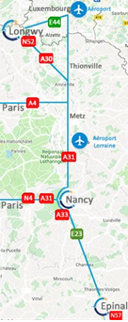
\includegraphics[width=0.3\linewidth]{f/planCRAN.png}
\caption{Plan d'accès et implantation du CRAN en France.}
\end{minipage}
\end{figure}

Au 1er janvier 2024, le CRAN comptait environ 250 membres :

\begin{itemize}
  \item 120 chercheurs ou enseignants-chercheurs (dont 8 chercheurs CNRS),
  \item des chercheurs de l'Institut de Cancérologie de Lorraine (ICL) du Centre Hospitalier Régional Universitaire (CHRU) ou d'organismes externes,
  \item 5 chercheurs émérites,
  \item 27 personnels administratifs et techniques,
  \item Environ 100 doctorants, ATER, post-doctorants et chercheurs invités.
\end{itemize}

Le laboratoire est organisé en trois départements scientifiques :

\begin{table}[h!]
\centering
\begin{tabularx}{\textwidth}{|C|C|}
\hline
\textbf{Département} & \textbf{Domaines principaux} \\ \hline
Contrôle, Identification et Diagnostic (CID) & Automatique, systèmes dynamiques \\ \hline
Modélisation, Pilotage et Sûreté des systèmes Industriels (MPSI) & Automatique, productique, génie informatique \\ \hline
Biologie, Signaux et Systèmes en Cancérologie et Neurosciences (BioSiS) & Biologie, neurologie, traitement du signal et de l'image \\ \hline
\end{tabularx}
\caption{Les différents départements du CRAN.}
\label{tab:cran}
\end{table}

\subsubsection{Le site de Longwy}

Mon stage s'est déroulé sur le site de l'IUT de Longwy, au sein du département Contrôle, Identification et Diagnostic (CID). Ce département compte actuellement 24 membres, dont :

\begin{itemize}
  \item 4 professeurs des universités dont 1 émérite,
  \item 5 maîtres de conférences,
  \item 1 ingénieur de recherche CNRS,
  \item 2 post-doctorants,
  \item 1 ATER,
  \item 4 doctorants,
  \item 8 stagiaires en master.
\end{itemize}

Les thématiques de recherche du département portent sur l'estimation, la commande et le diagnostic pour les systèmes avec des complexités spécifiques :

\begin{itemize}
  \item systèmes interconnectés en réseaux, 
  \item systèmes de grande dimension, 
  \item systèmes avec des paramètres incertains, 
  \item systèmes stochastiques.
\end{itemize}

Ces recherches trouvent des applications dans des domaines variés : 

\begin{itemize}
  \item véhicules autonomes et transports, 
  \item environnement et bio-procédés, 
  \item énergie, l'hydrogène ($H_2$) en particulière, 
  \item communications.
\end{itemize}

\newpage

\subsection{Définition du Sujet du Stage}

\subsubsection{Cahier des Charges Initial}

Le stage avait pour objectif de développer et valider des méthodes avancées d'observation d'état appliquées aux véhicules autonomes. Le cahier des charges initial incluait l'étude et la mise en œuvre de deux approches d'observations pour les systèmes non linéaires : les observateurs à grand gain (High-Gain Observers, HGO) et les observateurs à intervalle de temps fini (Fixed-Time LPV Observers, FLPV).

L'environnement de travail choisi était le simulateur CARLA, un environnement de simulation 3D \textit{open source} très utilisé par la communauté académique et scientifique. CARLA permet de reproduire des situations de circulation réelles (autoroutes, intersections, ...) et constitue ainsi une plateforme idéale pour exposer l'observateur à des situations proches de la réalité.

\begin{figure}[h!]
\centering
\begin{subfigure}[b]{0.25\textwidth}
    \centering
    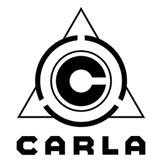
\includegraphics[width=\linewidth]{f/carla.png}
\end{subfigure}
\hfill
\begin{subfigure}[b]{0.65\textwidth}
    \centering
    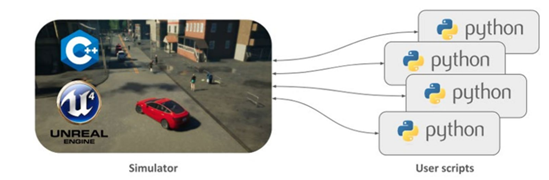
\includegraphics[width=\linewidth]{f/carlasim.png}
\end{subfigure}
\caption{Simulateur 3D CARLA.}
\label{fig:carla}
\end{figure}

Le stage devait se dérouler en plusieurs étapes :

\begin{itemize}
  \item Etude bibliographique et théorique : analyse des principes des observateurs HGO et FLPV et revue des défis en conduite autonome.
  \item Modélisation et implémentation : modélisation des véhicules dans CARLA, puis  implémentation des algorithmes d'observation HGO/FLPV en Python/C++.
  \item Interface utilisateur : développement d'un outil de visualisation permettant de configurer les observateurs, de suivre leur comportement en temps réel et d'analyser les résultats. Le cahier des charges initial envisageait une application de type Qt.
  \item Simulation complexe : La mise en place de scénarios complexes de simulation (suivi sur autoroute, navigation aux intersections, ...) afin d'évaluer la précision et la robustesse des méthodes étudiées.
  \item Documentation et recommandations : rédaction d'un rapport scientifique comprenant un guide méthodologique et les recommandations pour des applications réelles futures.
\end{itemize}

\subsubsection{Évolution du Sujet}

Au cours du stage, et après consultation des responsables du CRAN, le projet a été évolué afin de mieux s'adapter aux ressources et moyens techniques disponibles sur le site de Longwy et d'élargir la portée expérimentale du projet. Deux changements majeurs ont été apportés : le choix de l'environnement de test et la nature de l'interface utilisateur.

\subsubsection*{Environnement expérimental :}

Premièrement, au lieu de s'appuyer uniquement sur le simulateur CARLA, le stage a exploité les solutions de la société Quanser, à savoir le simulateur QLabs et le véhicule physique QCar2. Le simulateur QLabs offre une plateforme plus directement orientée vers l'enseignement et la recherche appliquée en automatique et en robotique. Il permet de tester rapidement des algorithmes dans un environnement virtuel simplifié mais réaliste, facilitant une itération rapide entre la théorie et pratique. Quant à QCar2, il s'agit d'un modèle de véhicule physique équipé de multiples capteurs (caméras, LIDAR, IMU, ...) et d'un système embarqué de calcul fonctionnant sous Ubuntu, ce qui facilite l'intégration avec des environnements logiciels tels que les bibliothèques de contrôle et de vision disponibles. Il est donc un support idéal pour passer de la simulation aux tests réels, tout en conservant un environnement contrôlé et sécurisé.

\begin{figure}[H]
\centering
\begin{minipage}[t]{0.9\textwidth}
\centering

\includegraphics[width=0.9\linewidth]{f/quanser.png}
\caption{Logo Quanser}
\end{minipage}
\end{figure}

\begin{figure}[H]
\centering
\begin{minipage}[t]{0.9\textwidth}
\centering
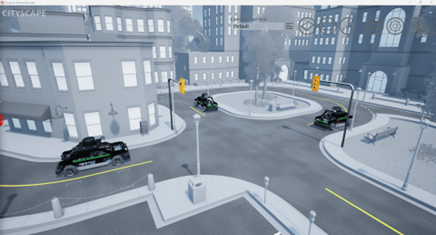
\includegraphics[width=0.9\linewidth]{f/qlabs_ex.png}
\caption{Simulateur QLabs}
\end{minipage}
\end{figure}

\begin{figure}[H]
\centering
\begin{minipage}[t]{0.9\textwidth}
\centering
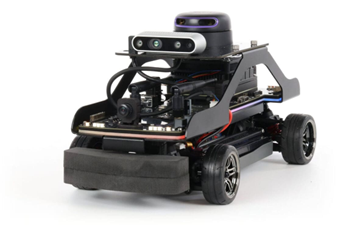
\includegraphics[width=0.5\linewidth]{f/qcar2.png}
\caption{QCar2}
\end{minipage}
\end{figure}

Ce passage de CARLA à QLabs et QCar2 a élargi la dimension expérimentale du projet, en validant les observateurs non seulement dans des scénarios virtuels mais aussi sur un véhicule physique.

\subsubsection*{Interface utilisateur :}

Deuxièmement, le développement de l'interface utilisateur a évolué vers une application web. Plutôt qu'une application de bureau locale en Qt, l'interface est conçue comme une application web interactive, accessible depuis un navigateur.

Cette solution présente plusieurs avantages :

\begin{itemize}
  \item Portabilité : Une fois qu'un navigateur moderne est installé, l'application est utilisable sur n'importe quel poste de travail sans installation complexe.
  \item Déploiement et partage : elle peut être hébergée sur un serveur dans un réseau local, permettant l'accès simultané par plusieurs utilisateurs.
\end{itemize}

L'application web permet de configurer les paramètres des observateurs, de suivre en temps réel les estimations produites et d'analyser visuellement leurs performances sur des scénarios simulés ou réels.

\begin{table}[h!]
\centering
\begin{tabularx}{\textwidth}{|p{3.5cm}|X|X|}
\hline
\multicolumn{1}{|c|}{\textbf{Aspect}} & 
\multicolumn{1}{c|}{\textbf{Cahier des charges initial}} & 
\multicolumn{1}{c|}{\textbf{Évolution du sujet}} \\ \hline

Environnement de test & Simulateur CARLA uniquement & QLabs (simulation) + QCar2 (véhicule physique) \\ \hline
Méthodes étudiées & Observateurs HGO et FLPV & Observateurs HGO et FLPV (inchangé) \\ \hline
Interface utilisateur & Application de bureau locale (Qt) & Application web interactive accessible via un navigateur \\ \hline
Validation & Scénarios simulés (autoroute, intersections, etc.) & Validation hybride : simulation + expérimentation réelle sur véhicule \\ \hline

\end{tabularx}
\caption{Tableau comparatif : Cahier des charges initial vs Évolution du sujet}
\label{tab:comparatif}
\end{table}

\newpage

\subsection{Description de l'Existant}

Avant le début de mon stage, les travaux menés portaient principalement sur l'étude théorique des méthodes d'observation d'état. Les principes des observateurs HGO et des observateurs FLPV avaient été largement étudiés sur le plan mathématique, et des résultats intéressants avaient déjà été obtenus au niveau de la modélisation et de l'analyse de leurs propriétés. 

Cependant, ces travaux restaient majoritairement confinés à des analyses théoriques et à des simulations numériques limitées, souvent réalisées dans des environnements de calcul simplifiés (scripts MATLAB...). Il manquait une étape essentielle : la validation expérimentale dans des environnements plus proches des conditions réelles.

Pour cela, deux plateformes étaient disponibles au laboratoire :

\begin{itemize}
  \item Le simulateur QLabs de Quanser, permettant de recréer un environnement virtuel réaliste où un véhicule autonome peut interagir avec son environnement. Cet outil offre la possibilité de tester des algorithmes dans des conditions variées comme le trafic, les obstacles, ...
  \item Le véhicule physique QCar2 de Quanser, un modèle de voiture connectée équipé de multiples capteurs (caméra, LIDAR, IMU, ...) et d'un système informatique intégré, est une plateforme pour passer de la simulation aux tests en conditions réelles et évaluer des observateurs dans des conditions physiques contrôlées.
\end{itemize}

Par conséquent, le cadre actuel présente un écart entre des résultats théoriques prometteurs et un manque de validation dans des environnements plus réalistes. L'intégration des observateurs HGO et FLPV n'a pas encore été implémentée dans QLabs ni dans QCar2. De plus, il n'existe aucune interface utilisateur permettant d'avoir un contrôle intuitif des observateurs et l'analyse de leurs performances.

Ce stage vise donc à combler le fossé entre théorique et pratique en assurant la mise en œuvre, l'intégration et la validation des observateurs sur les plateformes existantes.

\newpage

\subsection{Travail Effectué}

Cette section présente et met en valeur le travail effectué. La description technique détaillée du travail se trouve dans le rapport technique.

\subsubsection{Planification (Plan directeur)}

\subsubsection*{Plan initial}

Au début du stage, un plan directeur a été élaboré pour organiser le travail et prévoir les livrables associés. Ce document explique brièvement le contexte du stage et propose un plan couvrant la période d'avril à septembre 2025. 

\begin{figure}[h!]
\centering
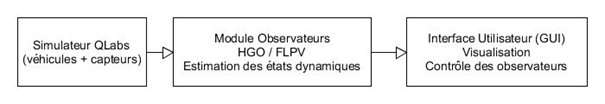
\includegraphics[width=0.9\textwidth]{f/context1.jpg}\\[1ex]
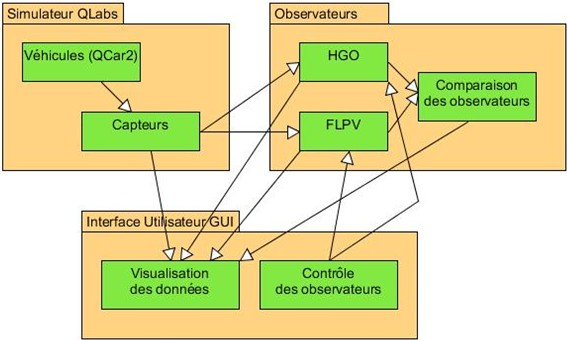
\includegraphics[width=0.9\textwidth]{f/context2.jpg}
\caption{Diagrammes de contexte.}
\label{fig:context}
\end{figure}

Les étapes principales prévues sont présentées dans le tableau ci-dessous :

\begin{table}[h!]
\begin{tabularx}{\textwidth}{|p{3.5cm}|X|X|}
\hline
\textbf{Période} & \textbf{Tâche principale} & \textbf{Livrables} \\ \hline

Avril 2025 & Prise en main de QLabs et ROS2 & Rapport de découverte et configuration \\ \hline
Mai 2025 & Prise en main du véhicule QCar2 physique et tests de la connectivité & Tests et configuration réseau \\ \hline
Juin 2025 & Intégration des observateurs avec QLabs & Module de test fonctionnel \\ \hline
Juillet 2025 & Développement de l'interface utilisateur GUI	& Prototype GUI \\ \hline
Août 2025 & Tests dans scénarios simulés et physiques & Résultats comparatifs, logs \\ \hline
Septembre 2025 & Analyse des performances, documentation complète & Rapport final, guide méthodologique \\ \hline

\end{tabularx}
\caption{Phasage du stage.}
\label{tab:plan_directeur}
\end{table}

\newpage

\subsubsection*{Evolution}

Au fur à mesure de l'avancement, mes responsabilités ont considérablement évoluées. Initialement centré sur l'intégration des observateurs, mon rôle a évolué vers des missions plus transversales liées à l'ingénierie logicielle. En effet, l'équipe dans laquelle j'ai travaillé disposait de compétences en automatique et en théorie des systèmes, mais avait peu d'expérience en informatique et en développement collaboratif.

Grâce à mon profil en ingénierie du développement logiciel, j'ai pris en charge :

\begin{itemize}
  \item Le développement du véhicule autonome (simulation dans QLabs et l'implémentation sur le QCar2 physique), afin de fournir une base prête à l'emploi sur laquelle les chercheurs pouvaient appliquer leurs algorithmes et observateurs.
  \item Un rôle de consultant informatique, fournissant un support technique quotidien à l'équipe pour résoudre des problèmes liés aux environnements, aux configurations réseau ou à la programmation.
  \item De mise en place d'une méthodologie de développement structurée, adaptée à une équipe peu familière avec les pratiques logicielles modernes
\end{itemize}

\subsubsection{Prise en main des environnements techniques}

Avant de commencer le développement, une étape importante est de comprendre et de se familiariser avec l'environnement logiciel et matériel utilisé pour le projet, notamment QLabs et ROS2, qui sont les plateformes de simulation et de communication des véhicules autonomes.

\subsubsection*{Présentation de ROS2}

ROS2 (Robot Operating System 2) est un \textit{middleware} largement utilisé dans la recherche et l'industrie robotiques. Il ne s'agit pas d'un système d'exploitation au sens classique, mais d'un ensemble de bibliothèques et d'outils facilitant le développement d'applications robotiques.

\begin{figure}[H]
\centering
\begin{minipage}[t]{0.9\textwidth}
\centering

\includegraphics[width=0.6\linewidth]{f/ros2_logo.png}
\caption{Logo ROS}
\end{minipage}
\end{figure}

Son rôle principal est d'assurer la communication entre les différents modules logiciels grâce à un mécanisme basé sur :

\begin{itemize}
  \item des nœuds : des processus indépendants représentant un capteur, un contrôleur ou un algorithme,
  \item des topics : les canaux de communication qui permettent l'échange de messages et des données en continu entre les nœuds, 
  \item des services : les appels synchrones entre les nœuds.
  \item ...
\end{itemize}

\begin{figure}[H]
\centering
\begin{minipage}[t]{0.9\textwidth}
\centering
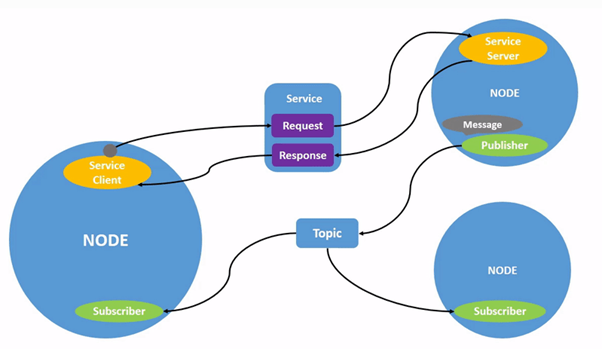
\includegraphics[width=1\linewidth]{f/ros2_comm.png}
\caption{Architecture de communication de base de ROS}
\end{minipage}
\end{figure}

Grâce à sa modularité, sa portabilité et sa capacité à s'intégrer à la fois aux robots physiques et aux environnements de simulation, ROS2 devient un outil essentiel pour le développement de véhicules autonomes.

\subsubsection*{Présentation de QLabs}

\textbf{Interface utilisateur et workspaces}

L'interface graphique de QLabs propose une navigation dans différents produits (robots développés par Quanser, ici on choisit QCar2) et différents \textit{workspaces} (espaces de simulation prédéfinis). Les différents workspaces correspondent à des environnements réalistes (zones urbaines, intersections, autoroutes, ...) dans lesquels il est possible d'instancier des objets virtuels.

Les icônes de l'interface utilisateur en haut de l'écran fournissent des commandes et des informations sur la caméra à l'utilisateur.

\begin{figure}[H]
\centering
\begin{minipage}[t]{0.9\textwidth}
\centering
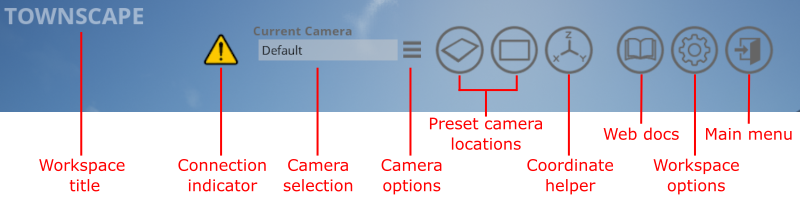
\includegraphics[width=\linewidth]{f/qlabs_user_interface.png}
\caption{Interface utilisateur QLabs}
\end{minipage}
\end{figure}

\begin{figure}[H]
\centering
\begin{minipage}[t]{0.9\textwidth}
\centering
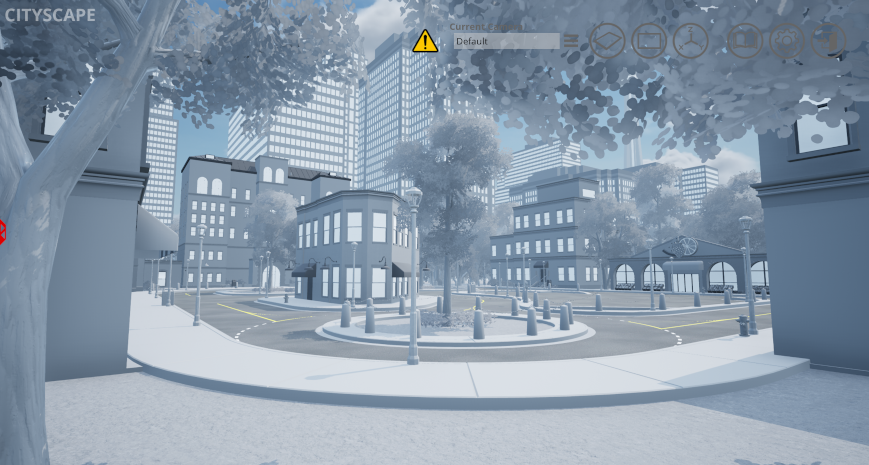
\includegraphics[width=\linewidth]{f/qcar_cityscape.png}
\caption{Exemple : Le workspace Cityscape}
\end{minipage}
\end{figure}

\begin{figure}[H]
\centering
\begin{minipage}[t]{0.9\textwidth}
\centering
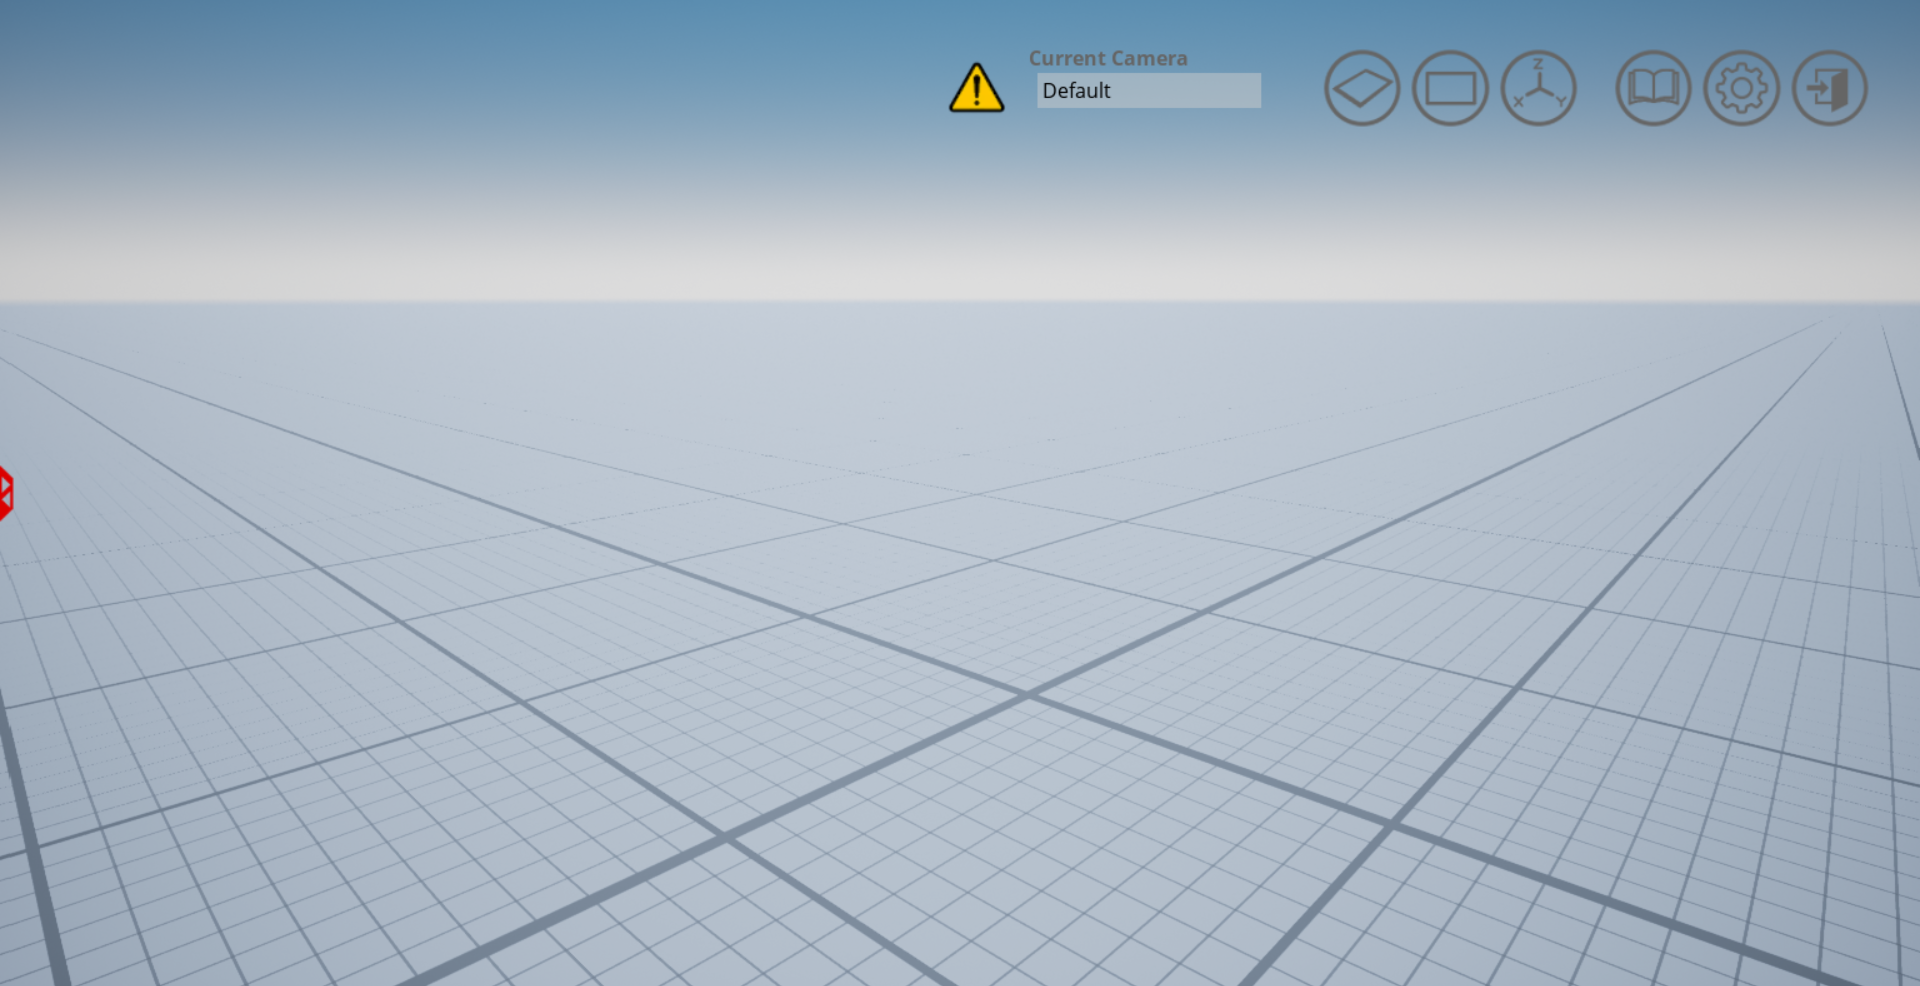
\includegraphics[width=\linewidth]{f/qcar_plane.png}
\caption{Exemple : Le workspace Plane}
\end{minipage}
\end{figure}

L'utilisateur peut : 

\begin{itemize}
  \item sélectionner un workspace et visualiser la scène 3D
  \item instancier des acteurs (véhicules, obstacles, piétons, ...)
  \item interagir avec la simulation (navigation libre dans l'environnement, caméra paramétrée, configuration de la scène, ...)
\end{itemize}

\textbf{Bibliothèques système}

D'après leur \textit{Design Philosophy} (philosophie de conception), QLabs n'est pas conçu pour être utilisé uniquement via l'interface utilisateur. Plutôt que d'interagir directement avec QLabs, Quanser fournit une bibliothèque dédiée en Python ainsi qu'un SDK (\textit{Software Development Kit}) permettant aux développeurs d'instancier et de contrôler des éléments de simulation.

La structure de ces bibliothèques est :

\begin{itemize}
  \item \textbf{QLabs Core} : fournir les fonctions de base pour initialiser la communication avec le simulateur et gérer les connexions.
  \item \textbf{System} : gérer l'interface utilisateur et le fenêtre de QLabs.
  \item \textbf{Real-Time} : lancer ou arrêter les modèles en temps réel conçu pour s'interfacer avec QLabs
  \item \textbf{Collection d'acteurs} : représenter des objets statiques ou dynamiques comme les véhicules (QCar2), les obstacles, les panneaux de signalisation, les piétons, …, et les instancie dans l'environnement.
  \item \textbf{Quanser SDK} : propose un ensemble d'outils et d'API facilitant le développement utilisant QLabs ou véhicule physique. Il fournit des pilotes de périphériques, des API en C et Python et des bibliothèques de communication et d'interfaces matérielles.
  \item etc.
\end{itemize}

\subsubsection*{Présentation de QCar2}

Le QCar2 est une plateforme mobile développée par Quanser pour l'enseignement et la recherche sur les véhicules autonomes. Il s'agit d'un véhicule connecté, à l'échelle 1/10, équipé d'un ensemble de multiples capteurs et d'actionneurs, et d'un puissant système embarqué, permettant la mise en œuvre de scénarios réalistes de conduite autonome et de développer, tester et valider des algorithmes d'observation.

\begin{figure}[H]
\centering
\begin{minipage}[t]{0.9\textwidth}
\centering
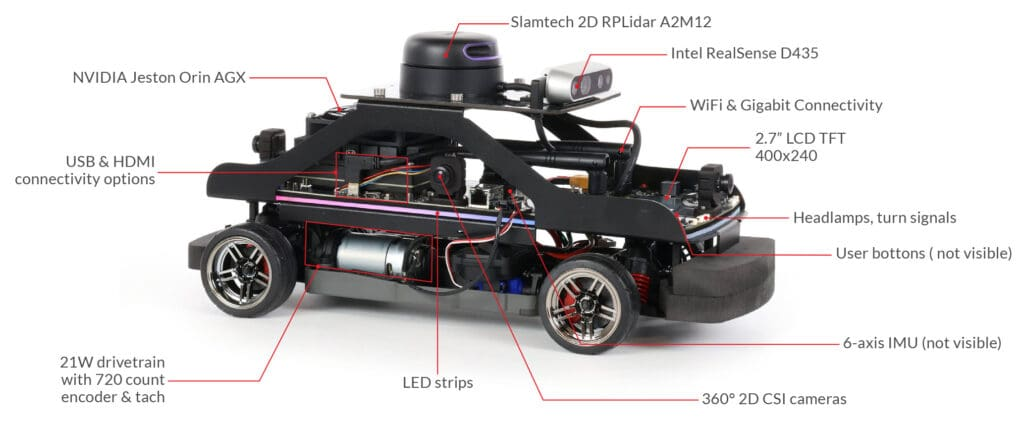
\includegraphics[width=0.9\linewidth]{f/qcar2schema.jpg}
\caption{Le QCar2 avec ses différents éléments.}
\end{minipage}
\end{figure}

\begin{itemize}
    \item \textbf{Unité de calcul} : NVIDIA Jetson Orin AGX, avec un ordinateur embarqué fonctionnant sous Ubuntu.
    \item \textbf{Capteurs de perception} : un LIDAR qui scanne l'environnement en 2D, une caméra 3D (Intel RealSense) pour la vision de profondeur, ainsi que quatre caméras panoramiques pour une vue à 360°.
    \item \textbf{Capteurs de navigation} : un capteur IMU 6 axes qui mesure les mouvements (accélérations et rotations) et des encodeurs de roue pour suivre précisément les déplacements.
    \item \textbf{Connectivité} : le véhicule peut communiquer via Wi-Fi ou câble Ethernet, et dispose de ports USB/HDMI pour le développement.
    \item \textbf{Interface} : un petit écran LCD, des boutons utilisateurs, ainsi que des phares et clignotants pour simuler un vrai véhicule.
\end{itemize}

Cette combinaison de capteurs et de puissance de calcul rend le QCar2 particulièrement adapté pour expérimenter des scénarios réalistes

\subsubsection*{Simulation du QCar2 dans QLabs}

Une partie importante a consisté à comprendre et mettre en place la simulation du véhicule QCar2 dans QLabs. J'ai consacré du temps à étudier le code source des bibliothèques QLabs et ROS2 fournies par Quanser. Cela m'a permis de comprendre en profondeur le fonctionnement interne du simulateur et de son intégration avec ROS2.

Le processus se déroule en plusieurs étapes : 

\begin{itemize}
  \item \textbf{Instancier l'acteur QCar2} : dans QLabs, on instancie un acteur représentant le véhicule QCar2 dans l'environnement virtuel.
  \item \textbf{Démarrage du modèle temps réel (rt model)} : une fois l'acteur instancié, un modèle temps réel est lancé. Ce modèle simule le comportement du véhicule et génère en continu les flux de données issus des capteurs (caméras , LIDAR, …)
  \item \textbf{Emission locale des données} : ces flux de données sont simulés sur les ports locaux de la machine exécutant l'application QLabs. Chaque capteur virtuel produit un flux comparable à celui du QCar2 réel.
  \item \textbf{Bibliothèque ROS2} : une bibliothèque ROS2 développée et fournie par Quanser, permet de récupérer ces données simulées et de les publier sur des topics ROS2 correspondants. Pour l'utilisateur, le QCar2 virtuel apparaît comme un vrai robot ROS2 avec ces capteurs accessibles en temps réel.
\end{itemize}

Grâce à cette architecture, QLabs offre une simulation fidèle et intégrée du QCar2, permettant de développer et tester des algorithmes avant de les déployer sur le véhicule physique.

\subsubsection*{Utilisation de Docker pour ROS2 et QLabs}

Docker est utilisé comme environnement principal de développement et d'exécution.

Concrètement :

\begin{itemize}
    \item Les \textit{builds} (compilation du code, génération des packages ROS2),
    \item Le lancement des nœuds ROS2 (localisation, perception, contrôle),
    \item L'exécution des scénarios de simulation et de communication avec QLabs/QCar2
\end{itemize}

ont été réalisés à l'intérieur d'un conteneur Docker préconfiguré.

Les avantages sont multiples :

\begin{itemize}
    \item \textbf{Reproductibilité, et isolation} : l'environnement est identique sur toutes les machines, ce qui évite les problèmes liés aux versions de bibliothèques ou aux différences de configuration système. Les dépendances logicielles (ROS2, Python, ...) restent isolées du système hôte, évitant les conflits.
    \item \textbf{Portabilité} : le conteneur peut être déployé facilement sur n'importe quel poste.
\end{itemize}

\begin{figure}[H]
\centering
\begin{minipage}[t]{0.9\textwidth}
\centering

\includegraphics[width=0.9\linewidth]{f/docker-logo-blue.png}
\caption{Docker}
\end{minipage}
\end{figure}

\subsubsection{Développement du véhicule autonome}

Une grande partie de mon stage consistait à développer un véhicule autonome fonctionnel, utilisable à la fois dans l'environnement de simulation QLabs et sur le véhicule physique QCar2. L'objectif était de créer une plateforme capable de se déplacer de manière autonome, afin que les chercheurs puissent appliquer et tester leurs algorithmes d'observation.

\subsubsection*{Environnement simulé}

Dans QLabs, le véhicule virtuel QCar2 est instancié dans workspace « Plan », avec l'environnement généré par le script fourni par Quanser.. Le modèle temps réel est également lancé, simulant la dynamique du véhicule et générant en continu des données issues de ses capteurs (lidar, caméras, GPS, IMU). Ces flux sont ensuite publiés dans ROS2 sous forme de topics.

\subsubsection*{Suivi de trajectoire avec Stanley Controller}

Le suivi de trajectoire est un élément central de la conduite autonome. Pour cette tâche, j'ai utilisé le Stanley Controller, dont l'implémentation est fournie par Quanser pour le QCar2.

Le Stanley Controller est un algorithme classique de robotique mobile, initialement développé à Stanford pour la voiture autonome "Stanley", vainqueur du DARPA Grand Challenge (2005). 

\begin{figure}[H]
\centering
\begin{minipage}[t]{0.9\textwidth}
\centering
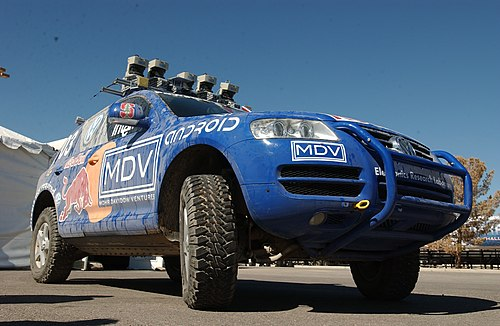
\includegraphics[width=0.9\linewidth]{f/Stanley2.jpg}
\caption{La voiture autonome Stanley}
\end{minipage}
\end{figure}

Il repose sur le principe suivant :

\begin{itemize}
  \item Le contrôleur calcule en continu l'erreur latérale (distance entre la position actuelle du véhicule et la trajectoire de référence).
  \item Il prend également en compte l'angle d'orientation du véhicule par rapport à la trajectoire.
  \item En combinant ces deux informations, il génère une commande de direction qui corrige la trajectoire du véhicule tout en assurant sa stabilité.
\end{itemize}

Dans le QCar2, l'implémentation fournie par Quanser permet un suivi robuste et précis des trajectoires planifiées dans QLabs. Mon rôle a consisté à intégrer ce contrôleur dans l'architecture ROS2 et à configurer les paramètres nécessaires.

\subsubsection*{Localisation}

Pour estimer la position du véhicule, j'ai utilisé l'approche combinant le GPS avec un filtre de fusion de données fourni par Quanser.

\textbf{GPS de Quanser basé sur le LIDAR}

En explorant le code source de la bibliothèque fournie par Quanser, j'ai constaté que la classe GPS n'exploite pas directement un capteur GPS physique classique. En réalité, elle lance un modèle temps réel spécifique (fichier \texttt{.rt-linux\_qcar2}) qui génère une estimation de position à partir des données du LIDAR.

L'implémentation interne de ce modèle n'est pas documentée, mais en analysant les appels de fonctions et les flux de données, j'ai identifié que la position est calculée à partir d'un traitement du LIDAR qui est une approche de \textit{Scan Matching} : les nuages de points générés par le LIDAR sont comparés pour estimer les déplacements du véhicule.

Ce “GPS” proposé par Quanser correspond en réalité à une estimation de la position, construite à partir des mesures du LIDAR, et imite le comportement d'un GPS standard.

\textbf{EKF}

Cet algorithme de filtrage EKF (\textit{Extended Kalman Filter}, ou filtre de Kalman étendu) est particulièrement adapté aux systèmes non linéaires comme le QCar2. Il repose sur deux étapes principales :

\begin{enumerate}
    \item Prédiction : l'état du véhicule (position, vitesse, orientation) est estimé à partir du modèle dynamique et des commandes appliquées (accélération, vitesse).
    \item Mise à jour : cette estimation est corrigée par les mesures issues du “GPS”.
\end{enumerate}

L'EKF combine les avantages de plusieurs sources :

\begin{itemize}
    \item le “GPS” Quanser,
    \item le modèle dynamique, qui fournit une estimation prédictive basée sur les commandes mais qui peut dériver avec le temps.
\end{itemize}

\subsubsection*{Évitement d'obstacles simplifié}

En plus du suivi de trajectoire et de la localisation, j'ai mis en place un système simplifié d'évitement d'obstacles basé sur les données LIDAR.

Le lidar du QCar2 produit un nuage de points représentant l'environnement proche. J'ai utilisé ces données pour construire une \textit{Occupancy Grid} (carte d'occupation), c'est-à-dire une grille qui indique quelles zones sont libres et quelles zones sont occupées par des obstacles.

\begin{itemize}
    \item Les zones grises représentent l'espace libre.
    \item Les pixels blancs correspondent aux cellules identifiées comme occupées (obstacles).
    \item Les segments bleus représentent les mesures du LIDAR, projetées dans l'espace pour détecter les obstacles autour du véhicule.
\end{itemize}

Cette carte constitue la base pour la perception de l'environnement : les données LIDAR fournissent la grille d'occupation, qui est ensuite utilisée par l'algorithme d'évitement pour adapter la trajectoire du véhicule.

\begin{figure}[H]
\centering
\begin{minipage}[t]{0.9\textwidth}
\centering
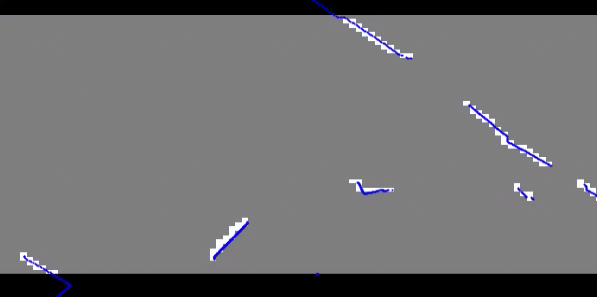
\includegraphics[width=0.9\linewidth]{f/occupancygrid.png}
\caption{Occupancy grid générée à partir des données LIDAR}
\end{minipage}
\end{figure}

L'algorithme, simplifié pour rester compatible avec les ressources disponibles, fonctionne ainsi :

\begin{itemize}
    \item génération de la grille à partir des données lidar,
    \item détection des cellules occupées devant le véhicule,
    \item modification locale de la trajectoire de référence afin d'éviter la zone détectée.
\end{itemize}

\subsubsection*{Architecture logicielle}

Le développement du véhicule autonome a reposé sur une architecture modulaire ROS2, dans laquelle chaque composant est implémenté sous forme de nœud indépendant. Cette approche garantit la flexibilité et facilite l'intégration d'algorithmes supplémentaires. L'architecture inclut :

\begin{itemize}
    \item des nœuds de localisation (GPS + EKF),
    \item des nœuds de perception (Occupancy Grid à partir du lidar),
    \item des nœuds de contrôle (suivi de trajectoire avec Stanley Controller).
\end{itemize}

\subsubsection{Support et rôle de consultant informatique}

En plus du développement technique, une part importante de mon travail est consacrée à un rôle de support informatique au sein de l'équipe. Le département CID possède des compétences en automatique et en théorie des systèmes, mais l'expérience des membres en développement informatique, de gestion de code et de configuration d'environnement complexes est limitée.

Dans ce contexte, j'ai joué le rôle de consultant informatique. Mes contributions ont été :

\begin{itemize}
    \item l'installation et la configuration de QLabs et ROS2 sur les différentes machines de l'équipe, incluant la gestion des dépendances, des environnements virtuels...,
    \item l'assistance dans le débogage des problèmes rencontrés lors de l'utilisation des bibliothèques Quanser ou des modules ROS2, 
    \item l'accompagnement des membres de l'équipe dans la prise en main de Git, de QLabs et de ROS2.
\end{itemize}

\subsubsection{Gestion du dépôt Git et stratégie de développement}

Dès le début, il est apparu que la gestion du code source constituait un point faible de l'organisation. Chaque membre de l'équipe travaillait de manière indépendante, avec peu de coordination. Cette approche rendait difficile l'obtention de résultats et l'intégration de contributions multiples.

\begin{figure}[h!]
\centering
\begin{subfigure}[b]{0.625\textwidth}
    \centering
    
\includegraphics[width=\linewidth]{f/logo git.png}
\end{subfigure}
\hfill
\begin{subfigure}[b]{0.275\textwidth}
    \centering
    
\includegraphics[width=\linewidth]{f/github logo.png}
\end{subfigure}
\caption{Git et GitHub.}
\label{fig:git}
\end{figure}

J'ai donc proposé et mis en œuvre une méthodologie structurée de gestion du code source, basée sur Git et GitHub. Le choix s'est porté sur une stratégie de \textit{Trunk-Based Development} (TBD), adaptée à une équipe pluridisciplinaire où la priorité est la simplicité et la rapidité d'intégration.

Les principes clés mis en place sont :

\begin{itemize}
    \item chaque membre de l'équipe développe sur une branch temporaire, dédiée à une tâche spécifique,
    \item une fois le développement teminé et validé, la branche est fusionnée dans la branche principale \texttt{main} via une \textit{Pull Request},
    \item l'utilisation de GitHub Project pour organiser les tâches, assigner des responsabilités et suivre l'avancement.
\end{itemize}

Afin de rendre cette méthodologie accessible à tous, j'ai rédigé un guide détaillé dans le fichier \texttt{README} du dépôt, incluant des instructions pas à pas sur :

\begin{itemize}
    \item la création de branches,
    \item la bonne pratique des commits,
    \item la gestion des \textit{Pull Requests},
    \item l'utilisation de GitHub Project pour la planification des tâches.
\end{itemize}

L'adoption de cette stratégie a permis d'instaurer une méthodologie collaborative claire et partagée. L'équipe a gagné en organisation et en traçabilité, et les nouveaux arrivants peuvent rejoindre le projet sans difficulté grâce à la documentation centralisée.

\begin{figure}[H]
\centering
\begin{minipage}[t]{0.9\textwidth}
\centering
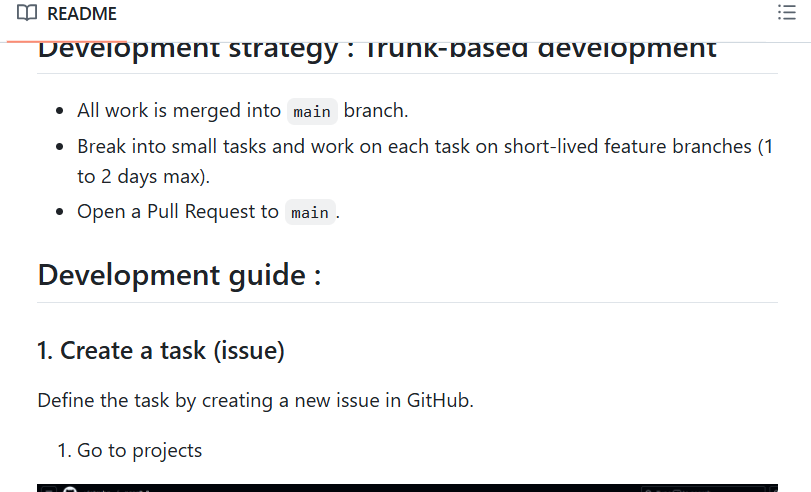
\includegraphics[width=0.9\linewidth]{f/readme.png}
\caption{Le fichier README.}
\end{minipage}
\end{figure}

\subsubsection{Développement de l'interface utilisateur}

Afin de faciliter l'utilisation du QCar2 et l'évaluation des observateurs, j'ai développé une interface utilisateur moderne sous forme d'une application Web. L'objectif était de rendre les expérimentations accessibles et intuitives, tout en garantissant une intégration fluide avec l'infrastructure logicielle existante.

\begin{figure}[H]
\centering
\begin{minipage}[t]{\textwidth}
\centering
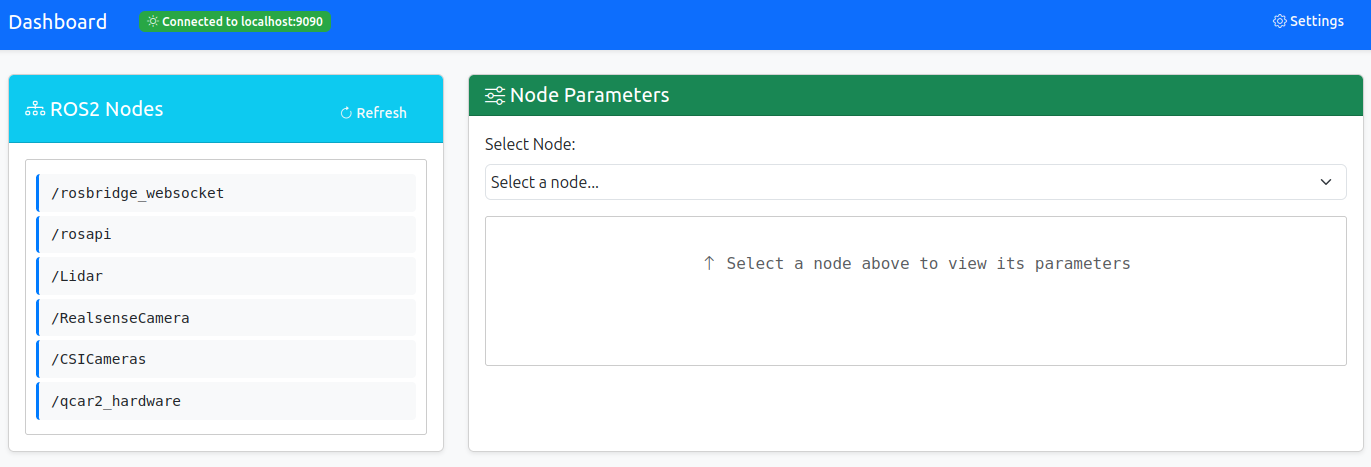
\includegraphics[width=\linewidth]{f/interfaceprototype.png}
\caption{Prototype d'interface utilisateur web.}
\end{minipage}
\end{figure}

\subsubsection*{Architecture technique}

L'application web repose sur une architecture simple mais efficace :

\begin{itemize}
    \item un serveur Express.js (Node.js) pour héberger et servir l'application web,
    \item la suite \texttt{rosbridge-suite} et la bibliothèque \texttt{roslibjs} de Robot Web Tools
    \begin{itemize}
        \item \texttt{rosbridge-suite} agit comme un serveur intermédiaire exposant ROS2 via WebSocket,
        \item \texttt{roslibjs}, utilisée côté navigateur, permet de communiquer avec rosbridge et de manipuler les éléments ROS2 (topics, paramètres, ...).
    \end{itemize}
\end{itemize}

Grâce à cette architecture, l'application web peut :

\begin{itemize}
    \item s'abonner à des topics ROS2 pour interagir avec le QCar2,
    \item modifier les paramètres des nœuds en cours d'exécution,
    \item recevoir et afficher en temps réel les flux de données du robot (capteurs, observateurs, ...).
\end{itemize}

\begin{figure}[H]
\centering
\begin{minipage}[t]{\textwidth}
\centering
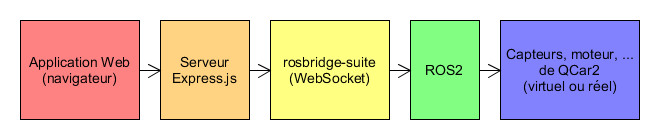
\includegraphics[width=0.9\linewidth]{f/arch.png}
\caption{Architecture de communication Application Web - ROS2 - QCar2.}
\end{minipage}
\end{figure}

\newpage

\subsection{Méthodologie}

\subsubsection{Organisation du travail}

Le programme de stage s'appuie sur un plan directeur prédéfini, qui définit les principales étapes : familiarisation avec l'environnement (ROS2, QLabs, QCar2), développement du véhicule autonome, intégration des observateurs et mise en œuvre des outils d'aide à l'utilisation de la plateforme. Ce plan sert de référence, mais est régulièrement ajusté en fonction 
\begin{itemize}
    \item des priorités de l'équipe,
    \item des difficultés rencontrées.
\end{itemize}

L'approche utilisée est itérative : chaque nouvelle fonctionnalité (véhicule autonome, interface web, ...) est développée et validée progressivement, par simulation dans QLabs et QCar2 physique.

\subsubsection{Méthodologie de développement logiciel}

Mon expérience en ingénierie logicielle m'a permis d'appliquer des méthodes structurées au sein de l'équipe :

\begin{itemize}
    \item utilisation de Git et GitHub pour le contrôle de version, avec une stratégie de \textit{Trunk-Based Development} facilitant l'intégration rapide des contributions,
    \item utilisation de branches temporaires et de Pull Requests pour garantir la qualité du code,
    \item documentation systématique des procédures dans un fichier README et mise en place d'un GitHub Project pour le suivi des tâches.
\end{itemize}

\subsubsection{Collaboration et support}

Un aspect important de la méthodologie a été la collaboration avec les membres de l'équipe. J'ai joué le rôle de référent informatique, en aidant à la configuration des environnements et en résolvant les problèmes techniques. Cette approche a amélioré la performance de l'équipe et contribué à renforcer la collaboration au sein du département.

\subsubsection{Outils utilisés}

Le projet a reposé sur un ensemble d'outils logiciels et matériels :

\begin{itemize}
    \item \textbf{Outils de développement logiciel} :
    \begin{itemize}
        \item Git et GitHub (gestion de versions et suivi de projet),
        \item Visual Studio Code,
        \item Python (langage principal pour ROS2),
        \item Docker,
        \item Node.js et Express.js (serveur de l'application web),
        \item roslibjs et rosbridge-suite (Robot Web Tools) pour la communication entre application web et ROS2.
    \end{itemize}
    
    \item \textbf{Outils de simulation et robotique} :
    \begin{itemize}
        \item QLabs (environnement de simulation réaliste développé par Quanser),
        \item QCar2 (plateforme robotique physique équipée de capteurs),
        \item ROS2 (\textit{middleware} de robotique pour la gestion des nœuds, topics, services).
    \end{itemize}
\end{itemize}

\newpage

\subsection{Difficultés rencontrées}

\subsubsection{Complexité des environnements logiciels}

L'une des premières difficultés a été la complexité de l'environnement ROS2 et des bibliothèques fournies par Quanser. L'installation et la configuration de ROS2 (dépendances, compatibilité avec le système d'exploitation) ont demandé un travail important de compréhension et de documentation.

\textbf{Solution retenue} : j'ai mis en place des environnements reproductibles et rédigé un guide pratique pour l'équipe, afin que chacun puisse configurer son poste de travail rapidement et éviter de répéter les mêmes erreurs.

\subsubsection{Documentation limitée des bibliothèques Quanser}

Les bibliothèques QLabs et QCar2 fournies par Quanser sont puissantes, mais leur documentation est parfois limitée. La compréhension de leur fonctionnement interne (exemple : GPS basé sur LIDAR et \textit{scan matching}) n'était pas toujours claire.

\textbf{Solution retenue} : j'ai analysé le code source fourni et expérimenté directement dans QLabs pour mieux comprendre le comportement des classes. J'ai ensuite partagé ces connaissances avec l'équipe, ce qui a permis de débloquer plusieurs travaux.

\subsubsection{Différences de compétences au sein du groupe}

Le projet s'est déroulé au sein d'une équipe aux compétences très variées : une forte expertise théorique en automatique, mais une expérience limitée en informatique et en gestion logicielle. De mon côté, ma formation et mon expérience étaient principalement orientées vers l'ingénierie logicielle, avec peu d'expérience en automatique et en robotique.

Cela a représenté un double défi :

\begin{itemize}
    \item aider mes collègues dans les aspects informatiques (développement logiciel, gestion de code, ...),
    \item tout en m'appropriant rapidement les notions de contrôle, de capteurs et de robotique mobile nécessaires pour comprendre le projet et contribuer efficacement.
\end{itemize}

\textbf{Solution retenue} : j'ai joué un rôle de référent informatique en formant mes collègues à Git, ROS2 et QLabs, et en instaurant une stratégie de développement claire (\textit{Trunk-Based Development}, GitHub Project). En parallèle, j'ai investi du temps dans l'auto-apprentissage de la robotique et de l'automatique (lecture de documentation, étude des bibliothèques Quanser, échanges avec les chercheurs), ce qui m'a permis de combler progressivement mes lacunes et de contribuer au développement du véhicule autonome.

\newpage

\subsection{Conclusion}

\subsubsection{Bilan du stage}

Ce stage m'a permis de travailler sur un projet informatique, robotique et automatique, dans un environnement de recherche exigeant.

\begin{itemize}
    \item Points positifs : 
    \begin{itemize}
        \item J’ai contribué de manière significative à la mise en place d’un développement collaboratif : gestion du dépôt Git, mise en place d’une stratégie de développement (\textit{Trunk-Based Development}), rédaction d’un guide d’utilisation pour les membres de l’équipe.
        \item J'ai acquis beaucoup d'expérience pratique avec ROS2 et l'écosystème Quanser (QLabs, QCar2)
        \item J'ai développé des modules pour le véhicule autonome : construction d'un \texttt{OccupancyGrid} avec LIDAR, intégration d'un contrôleur Stanley, logique simplifiée d'évitement d'obstacles.
    \end{itemize}
    
    \item Difficultés rencontrées : 
    \begin{itemize}
        \item Mon manque d'expérience initiale en automatique et en robotique m'a obligé à approfondir de nouveaux concepts (localisation, contrôleurs, observateurs d'état).
        \item Certains problèmes logiciels (par exemple la compatibilité des versions, ...) nécessitent du temps pour être compris et corrigés.
    \end{itemize}
\end{itemize}

\subsubsection{Perspectives}

Le travail effectué constitue une première étape vers une intégration complète des observateurs théoriques développés au CRAN dans un environnement expérimental. Plusieurs améliorations sont envisagées :

\begin{itemize}
    \item Implémenter et tester les observateurs HGO et FLPV dans QLabs, puis sur le QCar2 physique.
    \item Améliorer l’évitement d’obstacles en remplaçant la logique simplifiée actuelle par une planification plus avancée.
    \item Enrichir l'application web et ajouter plus de fonctionnalités, comme gérer plusieurs robots à la fois ...
\end{itemize}

\subsubsection{Conclusion générale}

Ce stage au CRAN a été pour moi une expérience très enrichissante, tant sur le plan professionnel que personnel. J'ai découvert un domaine nouveau - l'automatique et la robotique - dans lequel je n'avais que très peu d'expérience au départ. Cela m'a demandé un effort d'adaptation et d'apprentissage rapide, mais cette difficulté s'est transformée en une opportunité de développer de nouvelles compétences.

J'ai particulièrement apprécié de pouvoir mettre à profit mes connaissances en développement logiciel pour répondre à des besoins concrets de l'équipe : mise en place d'une méthodologie de travail collaborative, gestion d'un dépôt Git, conception d'une interface web intuitive. Jouer un rôle de référent informatique dans une équipe de chercheurs m'a permis de mesurer la valeur de mes compétences et de prendre confiance dans ma capacité à contribuer à des projets pluridisciplinaires.

Sur le plan personnel, cette expérience m'a appris à travailler en équipe avec des profils variés, à communiquer clairement avec des collègues aux compétences différentes des miennes et à m'adapter à un environnement de recherche.

En résumé, ce stage m'a permis non seulement d'acquérir de nouvelles compétences techniques, mais aussi de développer des qualités humaines telles que l'adaptabilité, la pédagogie et le travail en équipe.

\newpage

\subsection*{Références}

\begin{enumerate}
    \item Quanser. \textit{QLabs Virtual Environment Documentation}. \\\url{https://qlabs.quanserdocs.com/}
    \item Quanser. \textit{ACC Competition 2025}. \\\url{https://github.com/quanser/ACC-Competition-2025}
    \item Open Robotics. \textit{ROS2 Documentation}. \\\url{https://docs.ros.org/}
    \item NVIDIA. \textit{Isaac ROS Common Documentation}. \\\url{https://github.com/NVIDIA-ISAAC-ROS/isaac\_ros\_common}
    \item RobotWebTools. \textit{\texttt{rosbridge\_suite} and \texttt{roslibjs} Documentation}. \\\url{https://robotwebtools.github.io/}
\end{enumerate}

Outils d’IA utilisés : 

\begin{enumerate}
    \item OpenAI. ChatGPT. \url{https://chat.openai.com/}
    \item Anthropic. Claude AI. \url{https://claude.ai/}
    \item Google DeepMind. Gemini AI. \url{https://gemini.google.com/}
\end{enumerate}

\newpage

\section{Rapport technique}

\subsection{Prise en main des environnements}

La prise en main des environnements fournis par Quanser a représenté une étape essentielle pour comprendre la manière dont le simulateur QLabs, le véhicule QCar2 virtuel et les packages ROS2 interagissent.

Le projet est basé sur l'\textit{ACC Competition 2025} (\textit{American Control Conference}), une compétition annuelle organisée par Quanser.

\subsubsection{Environnements Docker utilisés par Quanser}

Quanser fournit deux conteneurs Docker pour séparer la simulation et le développement :

\begin{figure}[H]
\centering
\begin{minipage}[t]{\textwidth}
\centering
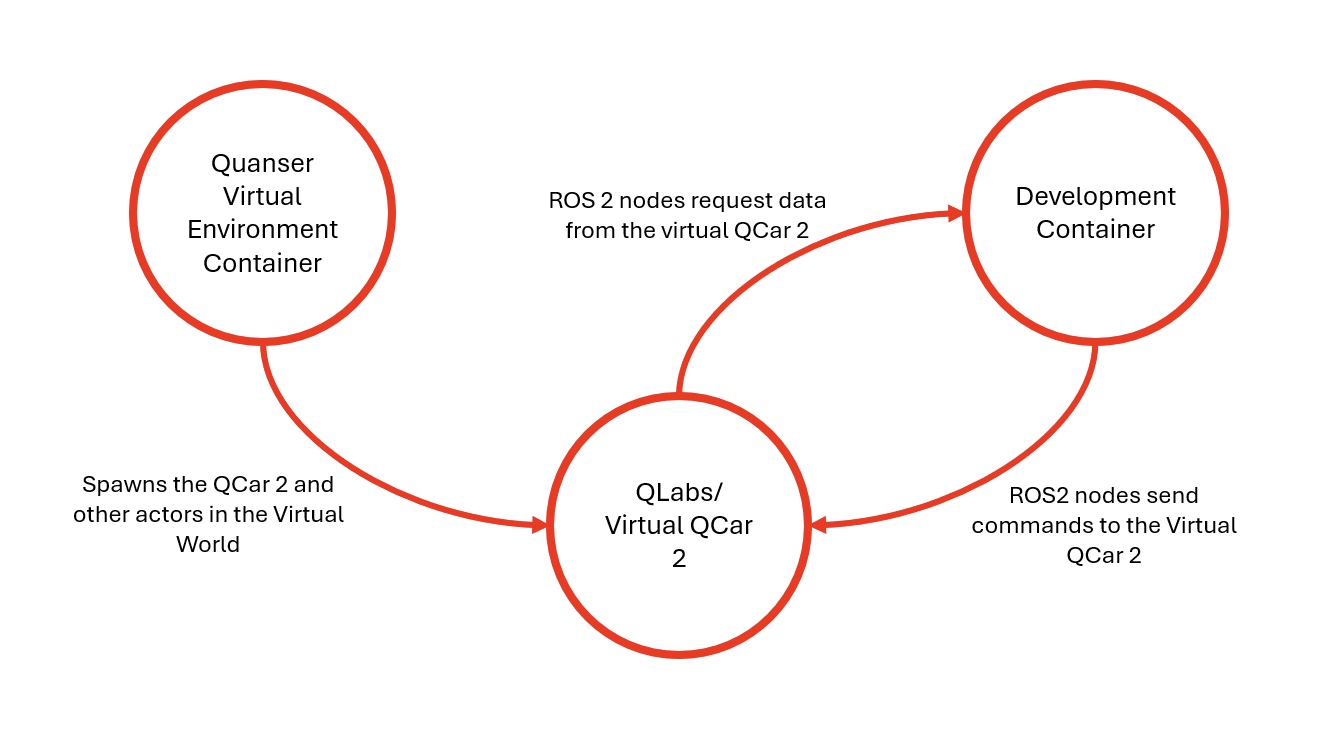
\includegraphics[width=0.9\linewidth]{f/simulation_graph.png}
\caption{Configuration de l’environnement virtuel QLabs avec les conteneurs Docker.}
\end{minipage}
\end{figure}

\begin{itemize}
    \item \textbf{Quanser Virtual Environment Container} : contient les scripts nécessaires à l'instanciation du QCar2 et des autres acteurs dans l'environnement virtuel. Le simulateur QLabs, exécuté sur la machine hôte, s'appuie sur ce conteneur pour gérer la scène 3D et les entités simulées.
    
    Par défaut, ces scripts sont intégrés directement dans l'image Docker, ce qui oblige à reconstruire l'image à chaque modification. Pour simplifier le développement, j'ai mis à jour le fichier Dockerfile et la commande de lancement du conteneur de manière à monter un dossier externe contenant mes scripts. Ainsi, les modifications de scripts sont prises en compte immédiatement sans avoir à reconstruire l'image, ce qui accélère considérablement les tests et les itérations.

    Construire un nouveau image avec la commande : \texttt{docker build -t my-virtual-qcar2 .}
    
    \texttt{sudo docker run --rm -it \textbackslash}
    
    \texttt{-v \$(pwd)/python:/home/qcar2\_scripts/python \textbackslash}
    
    \texttt{-v \$(pwd)/scripts:/home/qcar2\_scripts/scripts \textbackslash}
    
    \texttt{--network host \textbackslash}
    
    \texttt{--name my-virtual-qcar2 \textbackslash}
    
    \texttt{my-virtual-qcar2 bash}

    Utilisation de \texttt{-v} permet de monter les dossiers \texttt{python} et \texttt{scripts} du répertoire courant de l'hôte dans \texttt{/home/qcar2\_scripts/python} du conteneur à chaque lancement du conteneur.

    \item \textbf{Development Container} : contient l'environnement ROS2 Ce conteneur exécute l'environnement de développement basé sur ROS2. Quanser s'appuie sur l'infrastructure \textit{Isaac ROS Common}, un projet proposé par NVIDIA qui fournit des Dockerfiles et des scripts préconfigurés pour la création d'environnements de développement ROS2 optimisés.

    Dans notre dépôt, \textit{Isaac ROS Common} est intégré en tant que sous-module Git, initialement configuré en version \texttt{release-2.1}. Cependant, lors de mon stage, le conteneur de développement a cessé de fonctionner. Après plusieurs sessions de débogage, j'ai conclu que le problème provenait probablement de cette ancienne version d'\texttt{isaac-ros-common}.

    J'ai donc mis à jour le sous-module vers la version \texttt{release-3.2}, puis reconstruit le conteneur. Cette mise à jour a rétabli un environnement fonctionnel et stable, tout en assurant la compatibilité avec mes propres packages ROS2 développés.

    \texttt{cd /chemin/vers/isaac\_ros\_common}

    La commande pour lancer le conteneur Docker (ancienne version \texttt{release-2.1}):
    
    \texttt{./scripts/run\_dev.sh /chemin/vers/les/packages/ROS2}    
    
    Nouvelle commande (nouvelle version \texttt{release-3.2}):
    
    \texttt{./scripts/run\_dev.sh ---isaac\_ros\_dev\_dir /chemin/vers/les/packages/ROS2}

    Dans ce conteneur, on retrouve :
    
    \begin{itemize}
        \item les packages ROS2 fournis par Quanser,
        \item mes propres packages développés durant le stage. C'est donc dans ce conteneur que j'ai implémenté, lancé et validé les différents nœuds ROS2 utilisés pour le développement du véhicule autonome.
    \end{itemize}
\end{itemize}

\subsubsection{Simulation d'un QCar2 dans QLabs}

Le processus de lancement d'une simulation suit une séquence bien définie :

\textbf{1. Création de l'environnement et instanciation du QCar2}

Un script Python permet de générer l'environnement et un acteur QCar2 dans QLabs avec un identifiant unique.

\begin{lstlisting}[style=pythonstyle]
# Spawn a QCar at the given initial pose
car2 = QLabsQCar2(qlabs)
car2.spawn_id(actorNumber=0, 
            location=initialPosition, 
            rotation=initialOrientation,
            scale=[.1, .1, .1], 
            configuration=0, 
            waitForConfirmation=True)
\end{lstlisting}

\begin{figure}[H]
\centering
\begin{minipage}[t]{\textwidth}
\centering
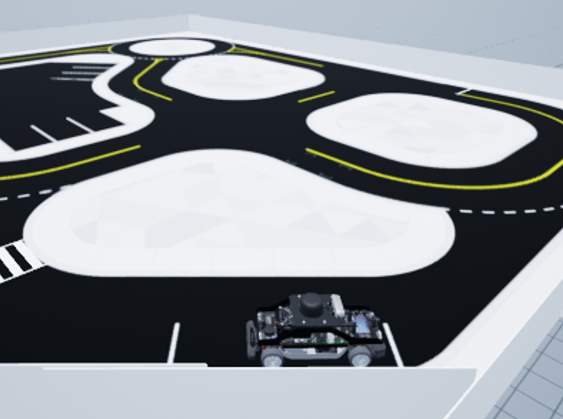
\includegraphics[width=0.9\linewidth]{f/qlabs_qcar2.png}
\caption{QCar2 (à l'échelle 1/10) dans simulateur QLabs.}
\end{minipage}
\end{figure}


\textbf{2. Lancement du modèle temps réel associé au QCar2}

Le modèle temps réel est démarré :

\begin{lstlisting}[style=pythonstyle]
rtModel = os.path.normpath(os.path.join(os.environ['RTMODELS_DIR'], 'QCar2/QCar2_Workspace_studio'))
QLabsRealTime().start_real_time_model(rtModel)
\end{lstlisting}

\begin{lstlisting}[style=pythonstyle]
def start_real_time_model(self, ...):

    ...
    cmdString="start \"QLabs_{}_{}\" \"%QUARC_DIR%\\quarc_run\" -D -r -t tcpip://localhost:17000 \"{}.rt-win64\" -uri tcpip://localhost:{} -hostname {} -devicenum {} {}".format(modelName, actorNumber, modelName, self._URIPort, QLabsHostName, actorNumber, additionalArguments)
    ...
    
    
    os.system(cmdString)
\end{lstlisting}

Ce modèle ouvre automatiquement plusieurs ports TCP (18960-18969) pour diffuser les données simulées des capteurs (caméra, LIDAR, ...).

\begin{figure}[H]
\centering
\begin{minipage}[t]{\textwidth}
\centering
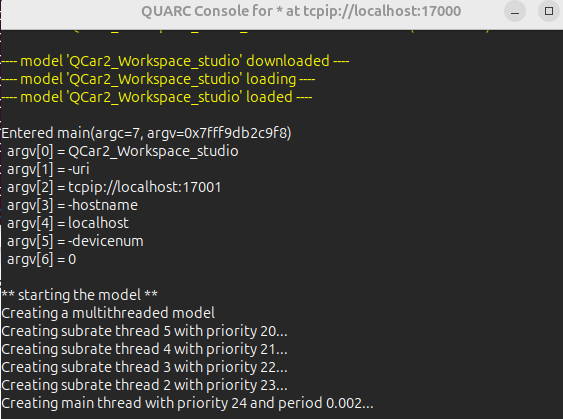
\includegraphics[width=0.9\linewidth]{f/qlabs_console.png}
\caption{Console QUARC.}
\end{minipage}
\end{figure}


\textbf{3. Vérification des ports ouverts par le modèle}

Pour confirmer que le modèle s'exécute bien et identifier les ports utilisés, on peut lister les processus et filtrer ceux liés au QCar2. La commande suivante affiche uniquement les connexions réseau du fichier \texttt{QCar2\_Wor} (correspondant au modèle lancé \texttt{QCar2\_Workspace\_studio}) :

\texttt{sudo lsof -i -P -n | grep QCar2\_Wor}

\begin{itemize}
    \item \texttt{lsof} (\textit{list open files}) : commande qui liste tous les fichiers ouverts par les processus.
    \item \texttt{-i} filtre les fichiers liés à des connexions réseau (TCP/UDP)
    \item \texttt{-P} affiche les numéros de ports au lieu de noms de ports
    \item \texttt{-n} affiche directement les adresses numériques (sans la résolution DNS des adresses IP)
    \item \texttt{grep QCar2\_Wor} : filtre la sortie pour ne garder que les lignes contenant \texttt{QCar2\_Wor}, correspondant au modèle en temps réel \texttt{QCar2\_Workspace\_studio}.
\end{itemize}

La sortie de cette commande liste les différents ports TCP/UDP utilisés par le modèle temps réel.

\begin{figure}[H]
\centering
\begin{minipage}[t]{\textwidth}
\centering
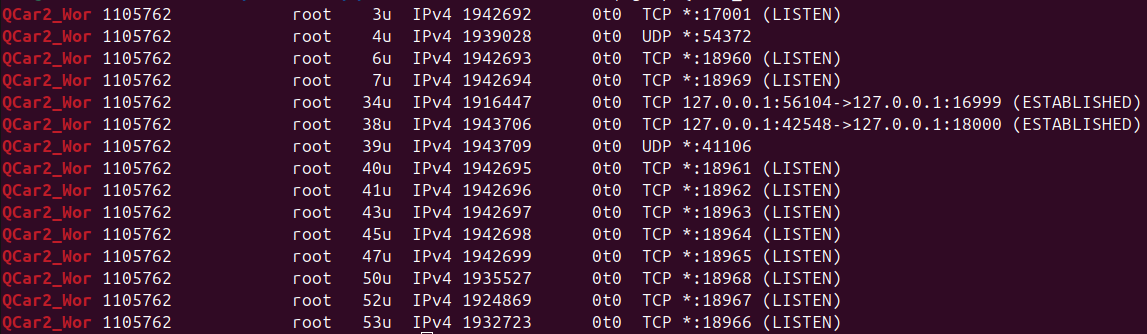
\includegraphics[width=0.9\linewidth]{f/capture_lsof.png}
\caption{Sortie de la commande \texttt{lsof}.}
\end{minipage}
\end{figure}


\textbf{4. Connexion ROS2 aux flux générés}

Les bibliothèques ROS2 de Quanser sont configurées pour se connecter aux ports exposés par le modèle temps réel à l'aide du Quanser SDK.

Par exemple l'URI utilisé pour récupérer les données de LIDAR dans le cas de véhicule virtuel (port 18966) et le cas de véhicule physique :

\begin{lstlisting}[style=pythonstyle]
if(device_type.compare("physical")==0){
    uri = "serial-cpu://localhost:1?baud='256000',word='8',parity='none',stop='1',flow='none',dsr='on'";
}
else if (device_type.compare("virtual")==0)
{
    uri = "tcpip://localhost:18966";

}
\end{lstlisting}

On obtient ce graphe dans \texttt{rqt\_graph} une fois les nœuds lancés.

\begin{figure}[H]
\centering
\begin{minipage}[t]{\textwidth}
\centering
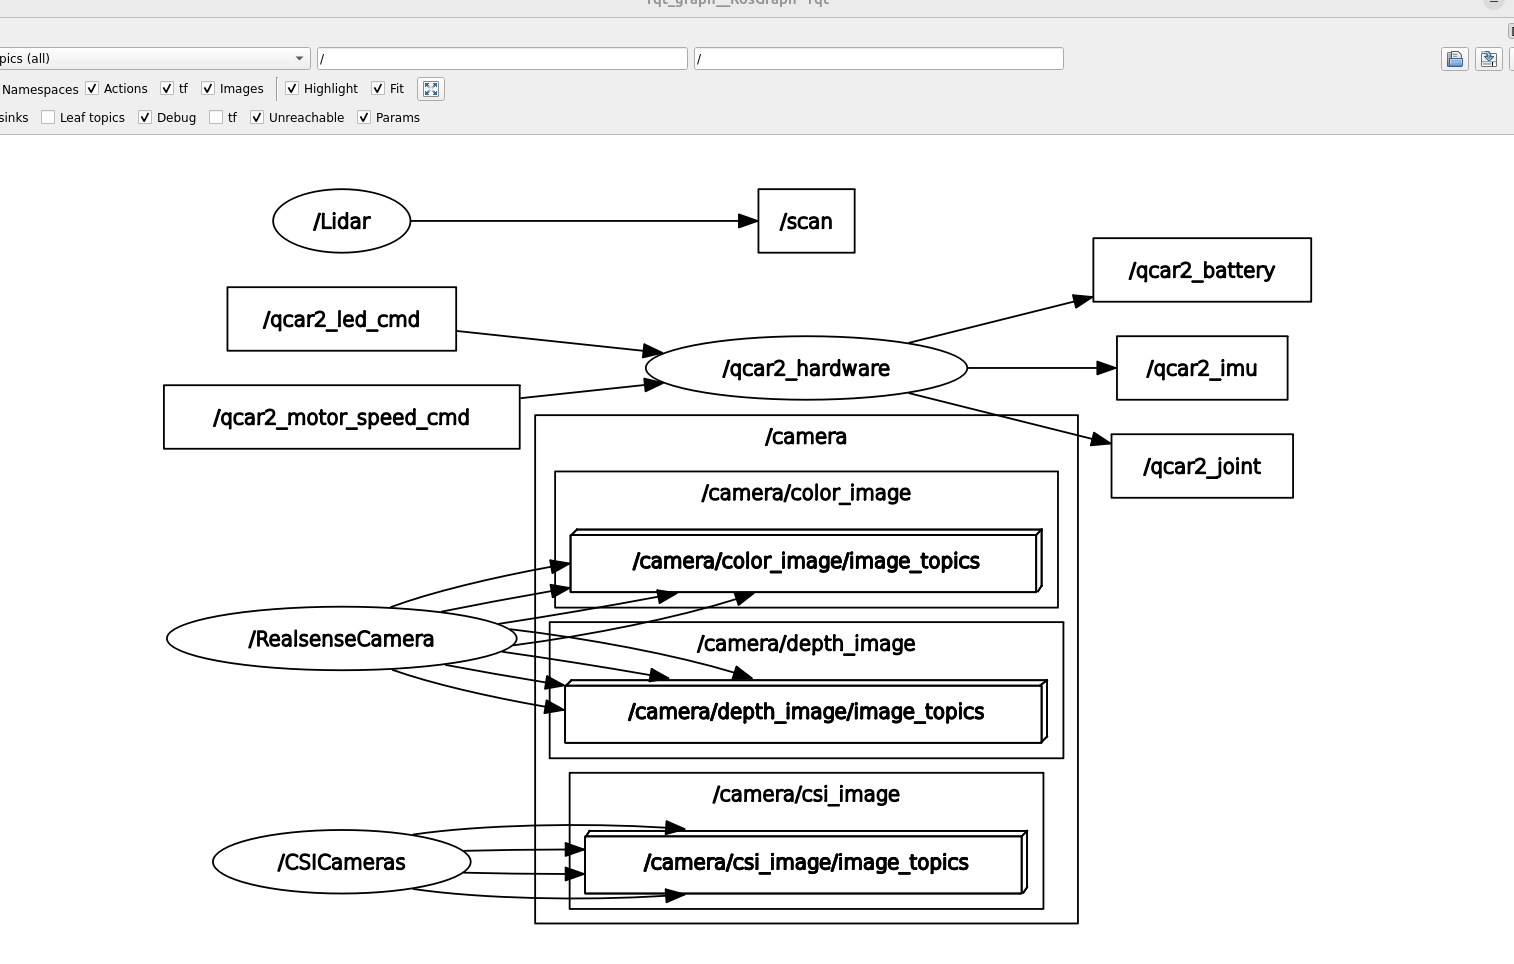
\includegraphics[width=0.9\linewidth, trim=0 0 0 6cm, clip]{f/qcarnodesgraph.png}
\caption{Graphe des nœuds et topics ROS2 de QCar2.}
\end{minipage}
\end{figure}

\subsection{Méthodologie de développement collaborative}

% \subsubsection{Structuration du dépôt et workflow collaboratif}

J'ai d'abord créé un dépôt GitHub unique afin de centraliser le code. Dans le README.md, j'ai listé les étapes à suivre pour :

\begin{figure}[H]
\centering
\begin{minipage}[t]{0.9\textwidth}
\centering
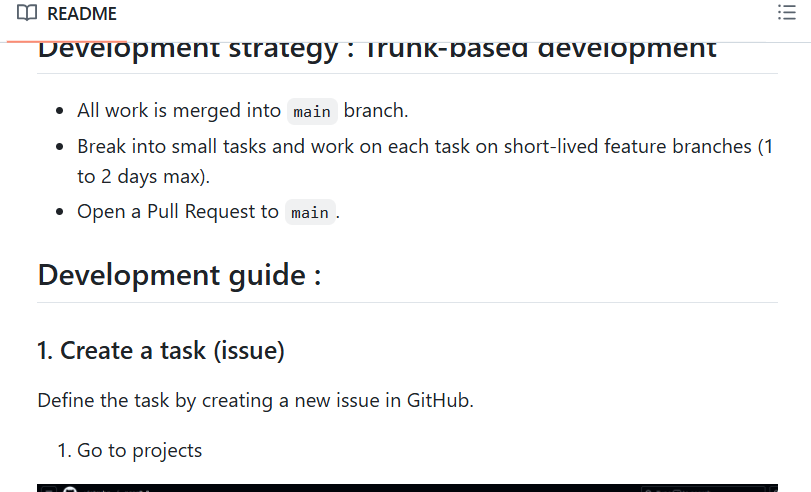
\includegraphics[width=0.9\linewidth]{f/readme.png}
\caption{Le ficher README.}
\end{minipage}
\end{figure}

\begin{itemize}
    \item Cloner et configurer l'environnement : commande git pour cloner le dépôt utilisant le jeton GitHub, configuration à faire, installation des logiciels nécessaires, commandes à exécutées pour lancer les conteneurs Docker.
    \item Organisation des branches : présentation de la stratégie du développement utilisée Trunk-Based Development :
    \begin{itemize}
        \item développement dans des branches courtes,
        \item intégration rapide via \textit{Pull Requests},
        \item garantie que la branche \texttt{main} reste toujours fonctionnelle.
    \end{itemize}
    \item Procédures Git : guide de développement détaillant le processus de développement étape par étape
    \begin{itemize}
        \item Aller au GitHub Project et créer une "issue" liée à sa tâche.
        \item Créer une branche temporaire pour travailler
        \item Appliquer les bonnes pratiques : branche courte durée, commits fréquents.
        \item Créer un \textit{Pull Request} et fusionner dans la branche \texttt{main}.
        \item Supprimer la branche temporaire.
    \end{itemize}
\end{itemize}

\subsection{Développement du véhicule autonome}

\subsubsection{Nœud \texttt{ekf.py} – Localisation}

Ce nœud met en œuvre l'EKF et le GPS fournis par Quanser afin d'estimer la pose du QCar2.

\textbf{Publication} : estimation de pose \texttt{PoseStamped} (position, rotation) publiée sur \texttt{/ekf\_pose} :

\begin{lstlisting}[style=pythonstyle]
self.pub_pose = self.create_publisher(PoseStamped, "/ekf_pose", 50)
\end{lstlisting}

\begin{lstlisting}[style=pythonstyle]
def publish_pose(self):
    msg = PoseStamped()
    # Recuperation des donnees de l'EKF
    ...
    self.pub_pose.publish(msg)
\end{lstlisting}

\textbf{Abonnements} :

Encodeurs (\texttt{/qcar2\_joint}) : vitesse calculée en m/s :

\begin{lstlisting}[style=pythonstyle]
self.sub_joint = self.create_subscription(JointState, '/qcar2_joint', self.joint_callback, 10)


def joint_callback(self, msg: JointState):
    self.motorTach = msg.velocity[0] * self.CPS_TO_MPS
\end{lstlisting}

IMU (\texttt{/qcar2\_imu}) : récupérer la vitesse angulaire z utilisée pour la prédiction :

\begin{lstlisting}[style=pythonstyle]
self.sub_imu = self.create_subscription(Imu, '/qcar2_imu', self.imu_callback, 10)


def imu_callback(self, msg: Imu):
    self.imu_data = msg.angular_velocity.z
    # mise a jour de l'EKF
    if self.imu_data:
        if self.gps.readGPS():
            # Recuperer les donnees GPS
            y_gps = ...
            
            self.ekf.update([self.motorTach, self.delta], dt, y_gps, self.imu_data)

        # si le GPS ne fournit pas de nouvelles donnees de mesure
        else:
            self.ekf.update([self.motorTach, self.delta], dt, None, self.imu_data)

    self.publish_pose()
\end{lstlisting}

\subsubsection{Nœud \texttt{lidar\_occupancy\_node.py} – Occupancy Grid}

Ce nœud transforme les mesures du LIDAR en une grille d'occupation exploitable par le contrôleur.

\textbf{Publication} : \texttt{OccupancyGrid} publiée sur \texttt{/occupancy\_grid} :

\begin{lstlisting}[style=pythonstyle]
self.occupancy_pub = self.create_publisher(OccupancyGrid, "/occupancy_grid", 10)


def publish_occupancy_grid(self):
    msg = OccupancyGrid()
    ...
    self.occupancy_pub.publish(msg)
\end{lstlisting}

\textbf{Abonnement} : \texttt{/scan} : données du LIDAR, utilisées pour remplir la grille puis la publier :

\begin{lstlisting}[style=pythonstyle]
self.subscription = self.create_subscription(LaserScan, '/scan', self.scan_callback, 10)


def scan_callback(self, msg: LaserScan):
    ranges = np.array(list(msg.ranges))[::-1]
    angles = np.linspace(msg.angle_min, msg.angle_max, len(ranges))
    self.populate_occupancy_grid(ranges, angles)
    self.publish_occupancy_grid()
\end{lstlisting}

\subsubsection{Nœud \texttt{vehicle\_control\_ros.py} – Contrôle et suivi de trajectoire}

Ce nœud est responsable du contrôle du véhicule.

\textbf{Publication} : envoyer des commandes moteurs (\textit{motor}, \textit{steer}) sur \texttt{/qcar2\_motor\_speed\_cmd} :

\begin{lstlisting}[style=pythonstyle]
self.motor_pub = self.create_publisher(MotorCommands, "/qcar2_motor_speed_cmd", 10)
\end{lstlisting}

\begin{lstlisting}[style=pythonstyle]
def send_control(self, motor, steer):
    msg = MotorCommands()
    ...
    self.motor_pub.publish(msg)
\end{lstlisting}

\textbf{Abonnements} :

\texttt{/ekf\_pose} : récupérer la localisation du véhicule, utilisée pour le suivi de trajectoire et l'évitement :

\begin{lstlisting}[style=pythonstyle]
self.ekf_sub = self.create_subscription(PoseStamped, '/ekf_pose', self.ekf_callback, 10)


def ekf_callback(self, msg: PoseStamped):
    pose = msg.pose
    x, y = pose.position.x, pose.position.y
    # calcul Stanley ou evitement selon occupancy grid
    ...
\end{lstlisting}

\texttt{/occupancy\_grid} : récupérer l'\textit{Occupancy Grid}, utilisé pour la détection d'obstacles :

\begin{lstlisting}[style=pythonstyle]
self.occupancy_sub = self.create_subscription(OccupancyGrid, '/occupancy_grid', self.occupancy_callback, 10)


def occupancy_callback(self, msg: OccupancyGrid):
    self.occupancy_grid = np.array(msg.data).reshape(msg.info.height, msg.info.width)
\end{lstlisting}

\textbf{Fonctionnalités principales} :

\textbf{1. Utilisation de Stanley Controller} : pour suivre une trajectoire planifiée :

\begin{lstlisting}[style=pythonstyle]
# generer la trajectoire
roadmap = SDCSRoadMap()
self.waypointSequence = roadmap.generate_path(self.nodeSequence)

# initialiser le controleur avec le trajectoire
self.stanleyController = StanleyController(
    waypoints=self.waypointSequence
)
\end{lstlisting}

Dans la boucle de contrôle :

\begin{lstlisting}[style=pythonstyle]
motor = self.speedController.update(...)

delta = self.stanleyController.update(x, y, yaw, v)
...
self.send_control(motor, delta)
\end{lstlisting}

\textbf{2. Évitement d'obstacles grâce à l'Occupancy Grid :}

Dans la boucle de contrôle, avant d'envoyer la commande de contrôle :

\begin{lstlisting}[style=pythonstyle]
if self.avoid_obstacle_occupancy_grid(...):
    return  # commande d'evitement envoyee
\end{lstlisting}

\textbf{3. Détection de collision – \texttt{check\_collision()}}

Cette méthode prend en entrée :

\begin{itemize}
    \item deux cellules : la position du véhicule et la cible actuelle (un point devant le véhicule sur la trajectoire),
    \item une marge de sécurité.
\end{itemize}

Le principe de cette méthode : trace les lignes sur la grille entre la position du véhicule et la cible et récupère les cellules traversées, pour chaque ligne elle applique un décalage latéral correspondant à la marge, et vérifie si ces lignes croisent une cellule occupée dans la grille.

\begin{lstlisting}[style=pythonstyle]
def check_collision(self, cell_a, cell_b, margin=0):
    for i in range(-margin, margin + 1):
        cell_a_margin = (cell_a[0], cell_a[1] + i)
        cell_b_margin = (cell_b[0], cell_b[1] + i)

        for cell in self.utils.traverse_grid(cell_a_margin, cell_b_margin):
            if self.occupancy_grid[cell] == self.IS_OCCUPIED:
                return True
    return False
\end{lstlisting}

\textbf{4. Génération d'une nouvelle cible}

Lorsque \texttt{check\_collision()} détecte une collision :

\begin{itemize}
    \item L'algorithme cherche une cible locale alternative autour de la trajectoire courante.
    \item Pour cela, il génère plusieurs points candidats décalés latéralement (de gauche à droite de la cible d'origine).
    \item Chaque point est testé avec \texttt{check\_collision()}.
    \item Le premier qui est libre est choisi comme nouvelle cible.
\end{itemize}

Une fois ce nouveau point trouvé :

\begin{itemize}
    \item le contrôleur calcule l'angle pour s'orienter vers ce point,
    \item une commande est envoyée avec \texttt{send\_control()}.
\end{itemize}

\begin{figure}[H]
\centering
\begin{minipage}[t]{\textwidth}
\centering
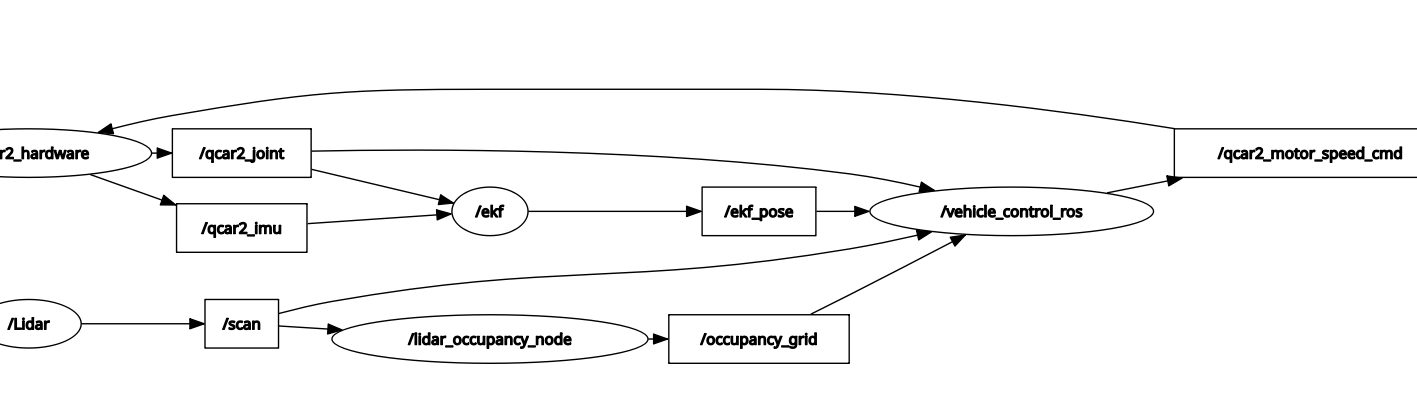
\includegraphics[width=0.9\linewidth]{f/vehiclecontrolgraph.png}
\caption{Graphe des échanges de données entre les nœuds.}
\end{minipage}
\end{figure}

Légende des symboles :

\begin{itemize}
    \item Ellipses ovales : représentent les nœuds ROS2.
    \item Rectangles : représentent les topics ROS2.
    \item Flèches : indiquent la direction du flux de données de nœud.
\end{itemize}

\begin{figure}[H]
\centering
\begin{minipage}[t]{\textwidth}
\centering
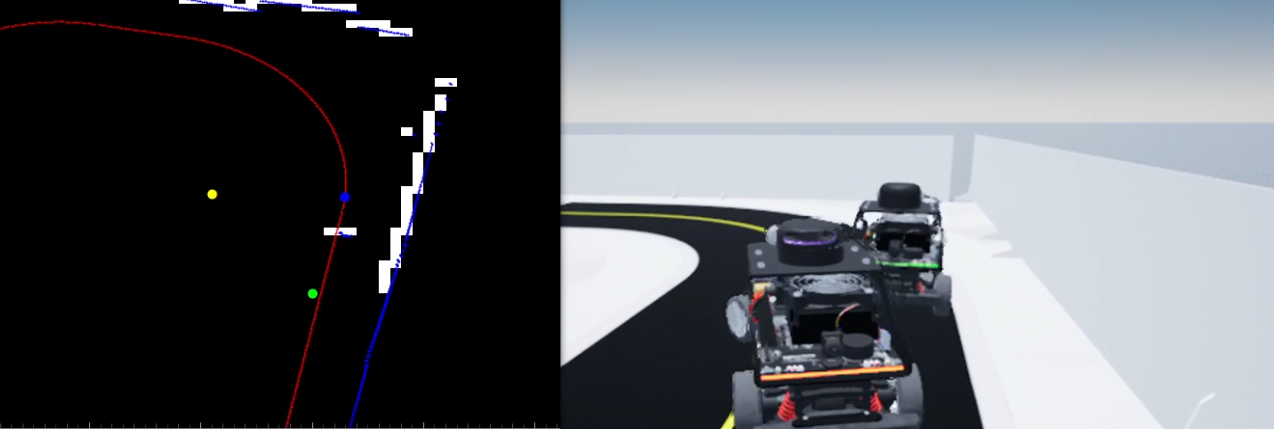
\includegraphics[width=0.9\linewidth]{f/avoidobstacle.png}
\caption{Evitement d'obstacle.}
\end{minipage}
\end{figure}


L'image ci-dessus illustre la prise de décision du contrôleur. Le point vert représente la position actuelle du véhicule. Le point bleu correspond à la cible initiale sur la trajectoire planifiée (points rouges). Les points bleus indiquent les mesures LIDAR, et les cellules blanches représentent les cellules occupées de l'\textit{Occupancy Grid}. Comme le chemin vers la cible est obstrué, le contrôleur génère une nouvelle cible locale (point jaune), permettant au véhicule de contourner l'obstacle.

\subsection{Développement d'une interface utilisateur (application web)}

\subsubsection{Architecture générale}

L'interface utilisateur web repose sur deux composants principaux : 

\begin{itemize}
    \item Un serveur Express.js : utilisé pour retourner les pages web (HTML, JavaScript, CSS). Il ne contient pas de logique complexe, mais sert à héberger et distribuer l’application.
    \item \texttt{rosbridge-suite} et \texttt{roslibjs} : la communication entre l’application et ROS2 s’effectue grâce au paquet \texttt{rosbridge-server} de \texttt{rosbridge-suite}, qui expose les nœuds, topics et services ROS2 via WebSocket, et à la bibliothèque JavaScript \texttt{roslibjs}, qui permet de récupérer l'information des nœuds, publier et souscrire directement aux topics depuis le navigateur.
\end{itemize}

\subsubsection{Architecture du code}

\textbf{Architecture Backend}

\texttt{server.js} : script principal pour configurer Express.js

\begin{itemize}
    \item Il sert les fichiers statiques (HTML, CSS, JavaScript)
    \item Il définit deux routes : 
    \begin{itemize}
        \item \texttt{/} : retourne \texttt{index.html} (Dashboard).
        \item \texttt{/settings} : retourne \texttt{settings.html} (page de configuration).
    \end{itemize}
\end{itemize}

\textbf{Architecture Frontend}

Le frontend emploie une architecture JavaScript modulaire avec une séparation claire des responsabilités :

\begin{enumerate}
    \item \texttt{main.js} : point d'entrée de l'application et initialisation.
    \item \texttt{config.js} : gestion de la configuration et constantes.
    \item \texttt{ros-connection.js} : gestion de la connectivité au serveur \texttt{rosbridge}.
    \item \texttt{node-list.js} : interface d'affichage et de sélection de nœuds.
    \item \texttt{node-parameters.js} : gestion des informations et mis à jour des paramètres de nœuds sélectionnés.
    \item \texttt{topic-subscriptions.js} : abonnements aux topics publiés par le nœud sélectionné.
    \item \texttt{message-visualizations.js} : Système de visualisation de messages reçu basé sur les classes.
    \item \texttt{event-handlers.js} : Gestion globale des événements.
    \item \texttt{settings-page.js} : Sauvegarde des préférences utilisateur et configuration dans \texttt{localStorage}.
\end{enumerate}

\subsubsection{Intégration de ROS2 avec \texttt{roslib.js}}

\textbf{Gestion des connexions}

\begin{itemize}
    \item Connexion WebSocket ROSBridge.
    \item Surveillance du statut de connexion avec indicateurs visuels.
    \item Paramètres de connexion configurables (hôte, port).
\end{itemize}

\begin{lstlisting}[style=pythonstyle]
// recuperer les parametres stockes dans localStorage
const ip = ... 
const port = ...
const url = `ws://${ip}:${port}`;
ros = new ROSLIB.Ros({
    url: url
});
\end{lstlisting}
    
\begin{figure}[H]
\centering
\begin{minipage}[t]{\textwidth}
\centering
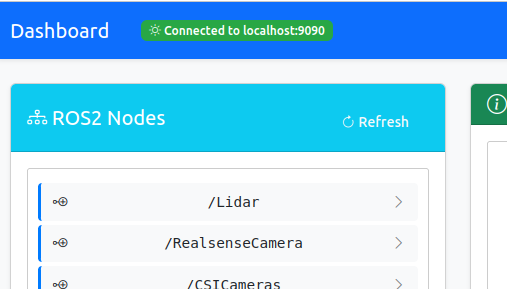
\includegraphics[width=0.6\linewidth]{f/ros-connection.png}
\caption{Indicateur visuel de statut de connexion.}
\end{minipage}
\end{figure}

\begin{figure}[H]
\centering
\begin{minipage}[t]{\textwidth}
\centering
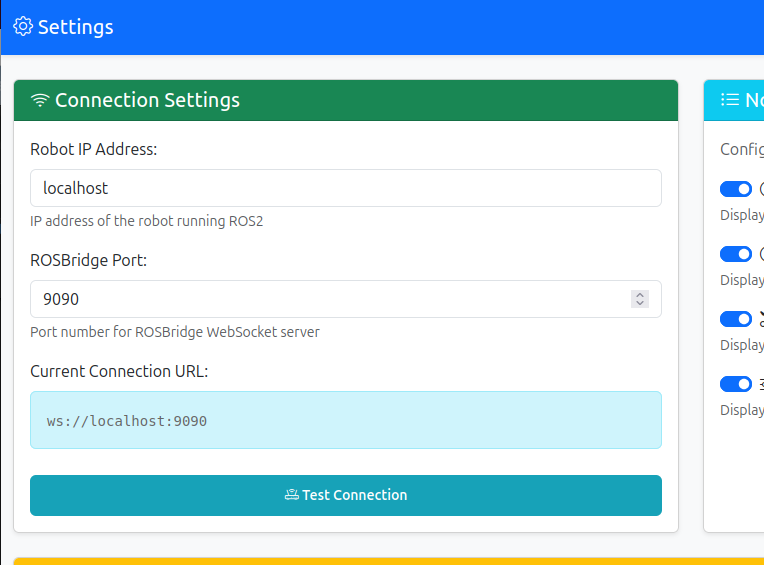
\includegraphics[width=0.6\linewidth]{f/setting-connection.png}
\caption{Paramètres de connexion ROSBridge.}
\end{minipage}
\end{figure}

\textbf{Gestion des nœuds}

\begin{itemize}
    \item Sélection interactive de nœuds : Interface de sélection basée sur les clics
    \item Affichage d'informations de nœuds : 
    \begin{itemize}
        \item Liste des topics abonnés
        \item Liste des topics publiés
        \item Services disponibles
        \item Paramètres éditables 
    \end{itemize}
\end{itemize}

La récupération des nœuds s'effectue via un appel de service. Le service est fourni par le nœud \texttt{rosapi} du serveur Rosbridge.

\begin{lstlisting}[style=pythonstyle]
const nodesClient = new ROSLIB.Service({
    ros: ros,
    name: '/rosapi/nodes',
    serviceType: 'rosapi/Nodes'
});
const request = new ROSLIB.ServiceRequest({});
nodesClient.callService(request, function(result) {
    ...
});
\end{lstlisting}

De même pour la récupération des informations du nœud :

\begin{lstlisting}[style=pythonstyle]
const detailClient = new ROSLIB.Service({
    ros: ros,
    name: '/rosapi/node_details',
    serviceType: 'rosapi/NodeDetails'
});
...
\end{lstlisting}

\begin{figure}[H]
\centering
\begin{minipage}[t]{\textwidth}
\centering
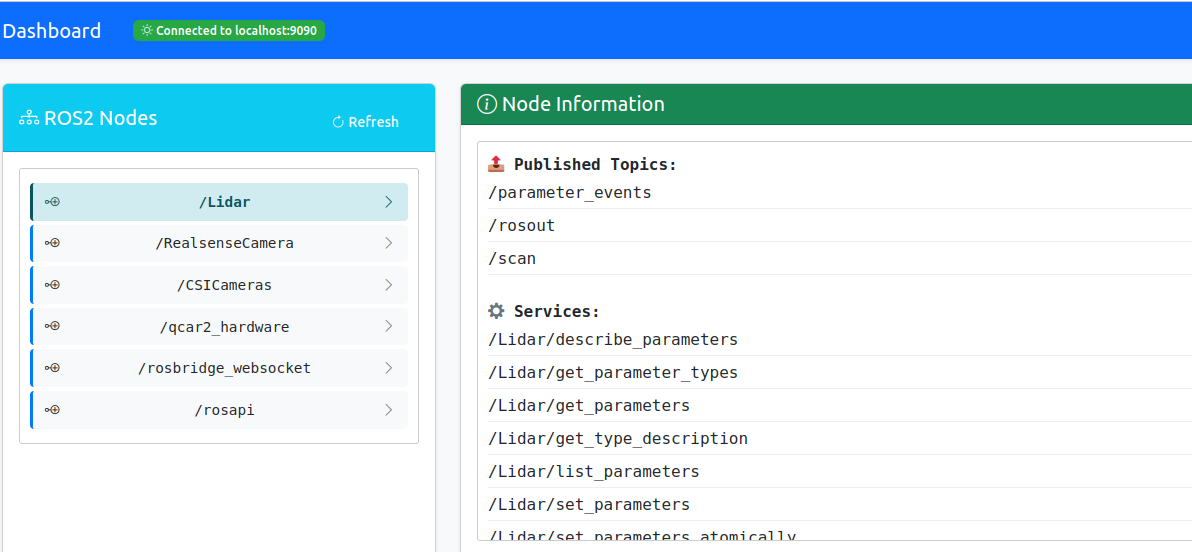
\includegraphics[width=\linewidth]{f/node-selection.png}
\caption{Affichage d’informations de nœuds sélectionnés.}
\end{minipage}
\end{figure}

La mise à jour des paramètres :

\begin{lstlisting}[style=pythonstyle]
const param = new ROSLIB.Param({
    ros: ros,
    name: paramName
});

param.set(newValue, function() {
    ...
})
\end{lstlisting}

\begin{figure}[H]
\centering
\begin{minipage}[t]{\textwidth}
\centering
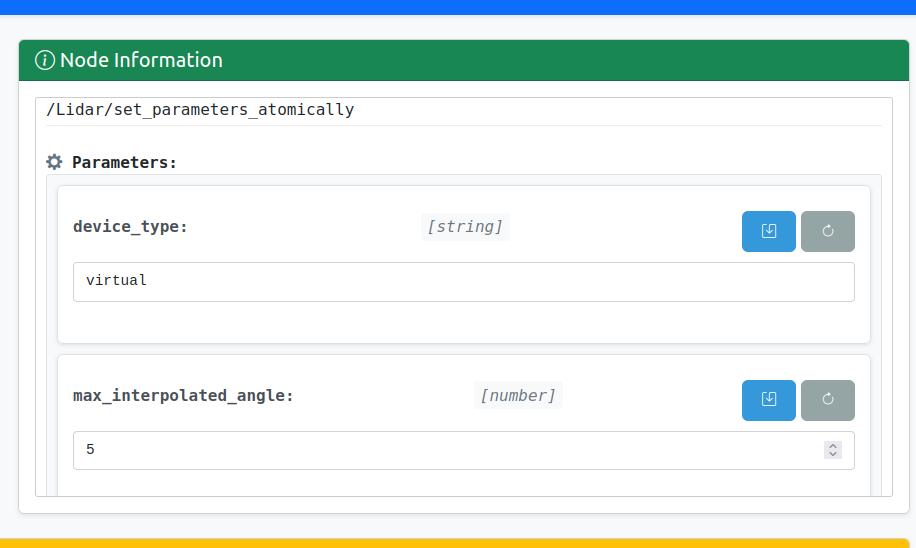
\includegraphics[width=0.8\linewidth]{f/parameter-update.png}
\caption{Mise à jour des paramètres du nœud sélectionné.}
\end{minipage}
\end{figure}

\begin{figure}[H]
\centering
\begin{minipage}[t]{\textwidth}
\centering
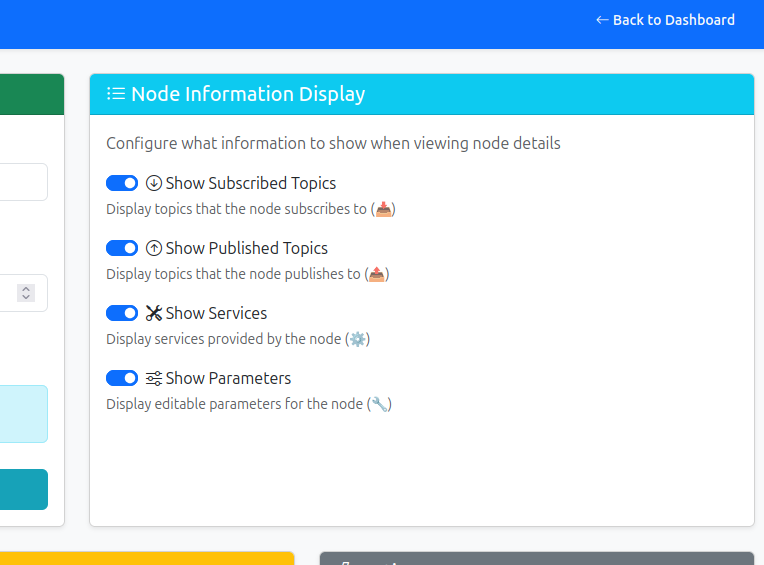
\includegraphics[width=0.8\linewidth, trim=0 4cm 0 0, clip]{f/setting-node.png}
\caption{Paramètres d'affichage du contenu des informations du nœud.}
\end{minipage}
\end{figure}

\textbf{Gestion d'Abonnement aux Topics}

\begin{itemize}
    \item Sélection de topic de nœud sélectionné à s'abonner et type de message.
    \item Gestion des topics abonnés et désabonnement.
\end{itemize}

\begin{lstlisting}[style=pythonstyle]
// stocker les abonnements aux topics actifs
let activeSubscriptions = new Map(); 


const listener = new ROSLIB.Topic({
    ros: ros,
    name: topicName,
    messageType: messageType
});
listener.subscribe(function(message) {
    // visualiser le message recu
}
activeSubscriptions.set(topicName, {
    listener: listener,
    messageType: messageType,
    startTime: new Date()
});
\end{lstlisting}

\begin{figure}[H]
\centering
\begin{minipage}[t]{\textwidth}
\centering
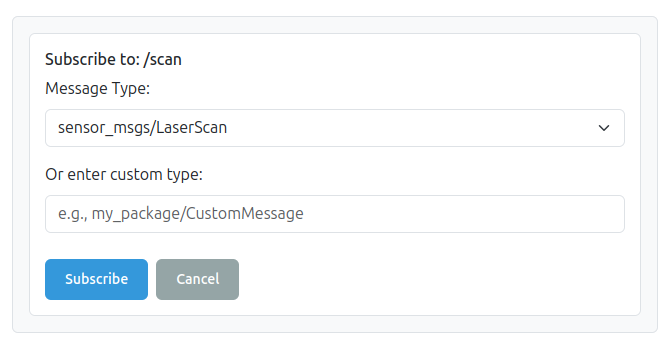
\includegraphics[width=0.8\linewidth]{f/message-type-selection.png}
\caption{Sélection de type de message.}
\end{minipage}
\end{figure}

\begin{figure}[H]
\centering
\begin{minipage}[t]{\textwidth}
\centering
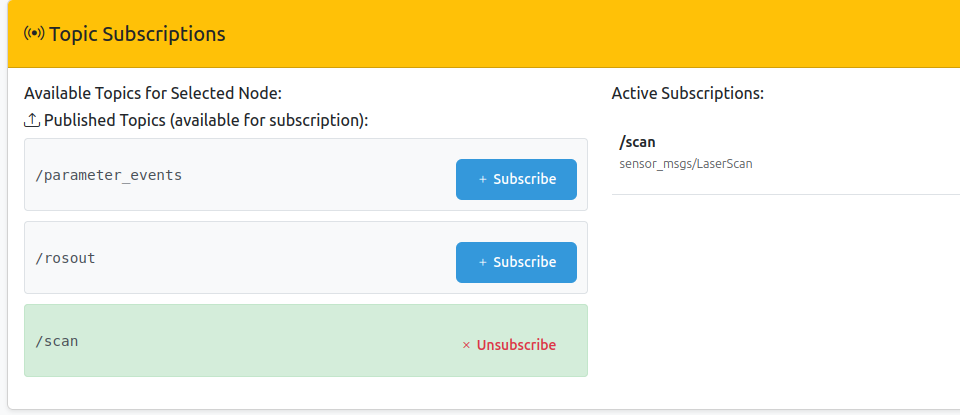
\includegraphics[width=\linewidth]{f/list-topic.png}
\caption{Liste des topics de nœud courant et les abonnement actifs.}
\end{minipage}
\end{figure}

\begin{figure}[H]
\centering
\begin{minipage}[t]{\textwidth}
\centering
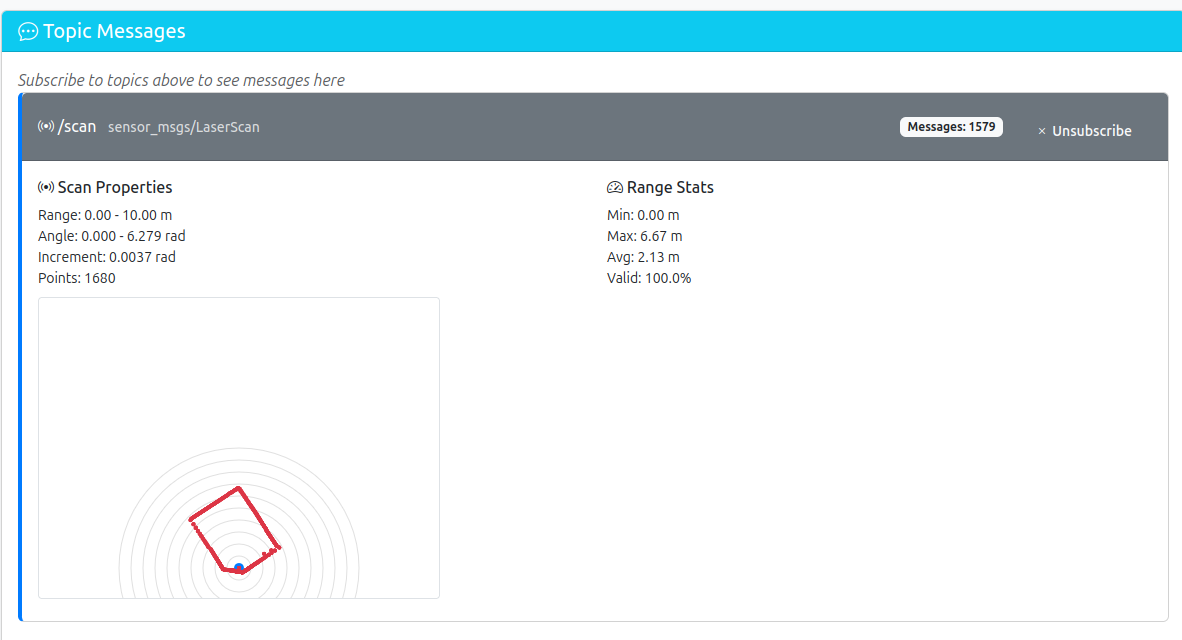
\includegraphics[width=\linewidth]{f/topic-scan.png}
\caption{Visualisation de message du topic \texttt{/scan}.}
\end{minipage}
\end{figure}

\begin{figure}[H]
\centering
\begin{minipage}[t]{\textwidth}
\centering
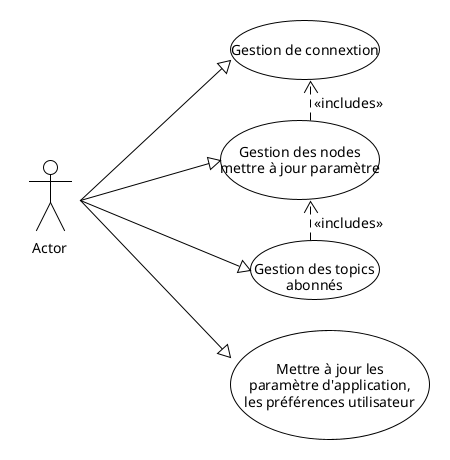
\includegraphics[width=0.6\linewidth]{f/usecase.png}
\caption{Diagramme de cas d'utilisation.}
\end{minipage}
\end{figure}

\subsubsection{Structure de visualisation de message}

Le système de visualisation de messages utilise une conception orientée objet avec héritage :

Classe de Base : \texttt{MessageVisualization}. 

\begin{itemize}
    \item Constructeur : Prend les paramètres "\texttt{vizId}", "\texttt{topicName}" et "\texttt{messageType}"
    \item Méthodes abstraites :
    \begin{itemize}
        \item \texttt{generateInitialHTML()} : générer un conteneur HTML pour ce type de message.
        \item \texttt{updateWithMessage(message)} : mettre à jour les éléments du conteneur avec le nouveau message.
    \end{itemize}
    \item Méthodes utilitaires :
    \begin{itemize}
        \item \texttt{getElement(elementId)} : récupération des éléments DOM
        \item \texttt{updateElement(elementId, content)} : mises à jour du contenu HTML interne
        \item \texttt{updateElementText(elementId, text)} : mises à jour du contenu texte
    \end{itemize}
\end{itemize}

Pour l'instant, il ne prend en charge que 3 types de message, les autres afficheront le message au format JSON par défaut.

\begin{itemize}
    \item \texttt{TwistVisualization} : \texttt{geometry\_msgs/Twist}.
    \item \texttt{LaserScanVisualization} : \texttt{sensor\_msgs/LaserScan}.
    \item \texttt{ImageVisualization} : \texttt{sensor\_msgs/Image}.
    \item \texttt{DefaultVisualization} : Affichage de messages génériques au format JSON.
\end{itemize}

\begin{figure}[H]
\centering
\begin{minipage}[t]{\textwidth}
\centering
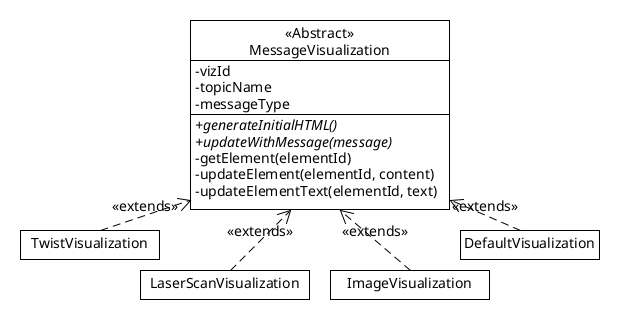
\includegraphics[width=\linewidth]{f/class-diag.png}
\caption{Diagramme de classe de structure de visualisation de message.}
\end{minipage}
\end{figure}

\begin{figure}[H]
\centering
\begin{minipage}[t]{\textwidth}
\centering
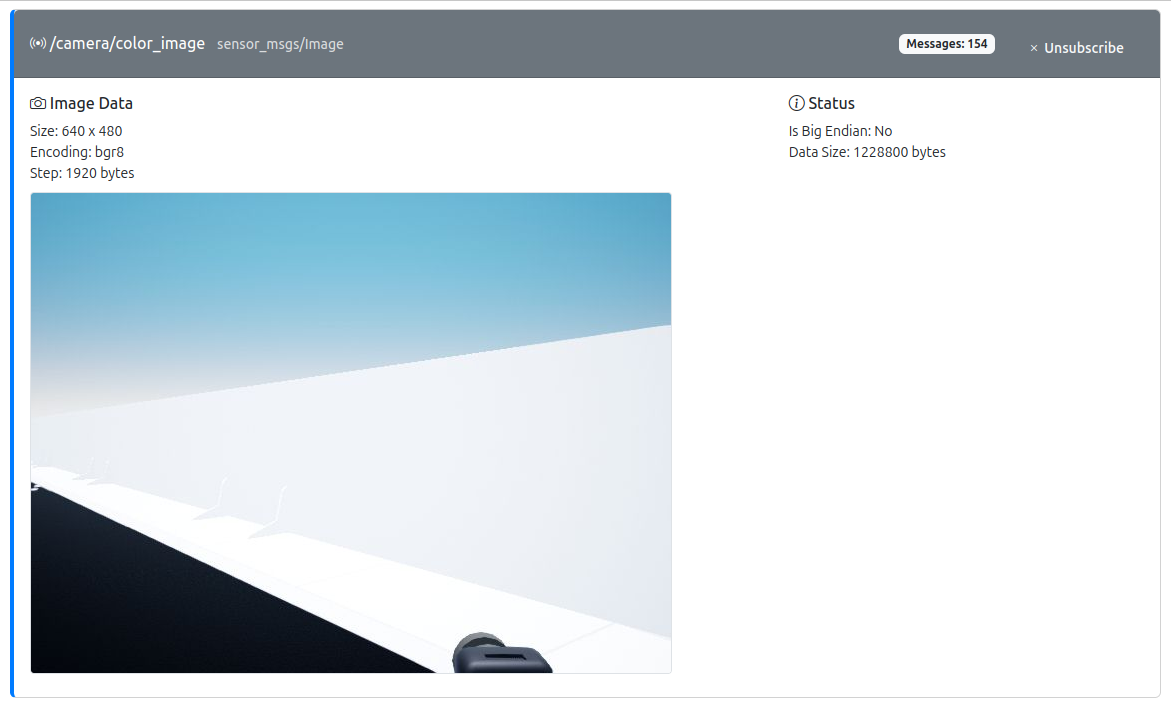
\includegraphics[width=\linewidth]{f/topic-image.png}
\caption{Visualisation de message du topic \texttt{/camera/color\_image} (classe \texttt{ImageVisualization}.}
\end{minipage}
\end{figure}

\end{document}